\documentclass{article}

\usepackage[english]{babel}
\usepackage[letterpaper,top=2.5cm,bottom=2.5cm,left=2.5cm,right=2.5cm,marginparwidth=1.75cm]{geometry}
\usepackage{amsmath, graphicx, tikz, pgfplots, multirow, newlfont, gensymb, indentfirst}

\usepackage{fancyhdr}
\pagestyle{fancy}
\fancyhf{}
\rhead{Jacob Sigman\\9/29/22}
\lhead{CE-344\\Environmental Systems Engineering}
\cfoot{\thepage}
\renewcommand{\headrulewidth}{1.5pt}
\setlength{\headheight}{22.6pt}
\usepackage[colorlinks=true, allcolors=black]{hyperref}
\setlength\parindent{24pt}

\begin{document}
    \begin{titlepage}
    \begin{center}
    {{\Large{\textsc{The Cooper Union for the Advancement of Science and Art}}}} \rule[0.1cm]{15.8cm}{0.1mm}
    \rule[0.5cm]{15.8cm}{0.6mm}
    {\small{\bf DEPARTMENT OF CIVIL AND ENVIRONMENTAL ENGINEERING}}\\
    {\footnotesize{STRUCTURAL ENGINEERING LABORATORY}}
    \end{center}
    \vspace{15mm}
    \begin{center}
    {\large{\bf LAB 5\\}}
    \vspace{5mm}
    {\Large{\bf COMPRESSIVE TESTING OF\\}}
    \vspace{2mm}
    {\Large{\bf STANDARD CONCRETE CYLINDER}}
    \end{center}
    \vspace{35mm}
    \par
    \noindent
    \hfill
    \vspace{20mm}
    \begin{center}
    {\large{ {\bf Group 2} \\ { Jenna Manfredi\hspace{5mm}David Madrigal\hspace{5mm}Gila Rosenzweig\\Nicole Shamayev\hspace{5mm}Jake Sigman}}}
    \vspace{40mm}
    {\large {\bf \\CE-321 \\ 12/14/22 \\}}
    \vspace{15mm}
    {\normalsize{Professor Tzavelis \\ Avery Kugler \\ Lionel Gilliar-Schoenenberger \\ Crystal Woo}}
    \end{center}
\end{titlepage}
    \tableofcontents
    \newpage
    \listoftables
    \addcontentsline{toc}{section}{List of Tables}
    \listoffigures
    \addcontentsline{toc}{section}{List of Figures}
    \newpage
    \section{Purpose of the Experiment}
    The purpose of this experiment is to determine the best method of recovering metal from sludge. The first goal is to determine the best method for separating water from sludge. The three methods to be analyzed are freeze/thaw, acidification, and centrifugation. The second goal is to compare the titration curves of various acid samples to determine which acid is the most efficient in lowering the pH of sludge. The third goal is to observe mixing times for samples with varying acids and levels of pH and determine the optimal mixing time and acid for removing lead. This experiment will provide all necessary and optimal aspects of recovering metals from sludge.
    \newpage
    \section{Procedure}
    \subsection{Freeze/Thaw}
    The separation of water from sludge is done in three ways: freeze/thaw, acidification, and centrifugation. The original water sample used contains 2\% solid and 98\% water, as seen in \textit{Figure 1}. After each process, the percentages of solid and water will be recalculated. In the freeze/thaw process, the solids are removed by freezing the sample. As the water freezes, the solids will separate from the water since water has a lower freezing point. As the solution thaws, since water has a higher melting point, the water will melt first, and will be left with substantially less solids remaining.
    \subsection{Acidification}
    In the acidification process, three different acids are used from three different labeled beakers. The three acids are sulfuric acid, nitric acid, and acetic acid. The acid is titrated into each beaker, and at various levels of concentration, the pH is recorded. Acid is added until the sample reached a pH of approximately 1.5 or if the normalization is too high to continue.
    \subsection{Centrifugation}
    In the centrifugation process, four groups are analyzed. Group A uses sulfuric acid with a pH of 1.5 at various mixing times. Group B uses sulfuric acid with a pH of 2 at various mixing times. Group C uses nitric acid with a pH of 1.5 at various mixing times. Group D uses sulfuric acid with a mixing time of six hours with various pH levels. These four groups are centrifuged and the percent removal of lead is recorded.
    \newpage
    \section{Data and Results}
    \section{Results}
\subsection{Varying $n$ Values}
\begin{center}


\addcontentsline{lot}{table}{Table 1: Initial $n$ Values}
\begin{tabular}{|c|cccccc|} 
    \hline
    \textbf{Station} & $n_1$ & $n_2$ & $n_3$ & $n_4$ & $n_5$ & $n_6$  \\ 
    \hline
    5.99             & 0.1      & 0.14     & 0.04     & 0.14     & -        & -         \\
    5.875            & 0.1      & 0.12     & 0.04     & 0.14     & -        & -         \\
    5.76             & 0.1      & 0.04     & 0.14     & -        & -        & -         \\
    5.685            & 0.09     & 0.1      & 0.04     & 0.1      & -        & -         \\
    5.61             & 0.08     & 0.1      & 0.04     & 0.06     & -        & -         \\
    5.525            & 0.07     & 0.09     & 0.1      & 0.04     & 0.06     & -         \\
    5.44             & 0.06     & 0.1      & 0.04     & 0.06     & -        & -         \\
    5.41             & 0.15     & 0.25     & 0.04     & 0.15     & -        & -         \\
    5.4              & -        & -        & -        & -        & -        & -         \\
    5.39             & 0.15     & 0.2      & 0.04     & 0.2      & 0.15     & 0.2       \\
    5.29             & 0.04     & 0.06     & 0.04     & 0.06     & -        & -         \\
    5.21             & 0.07     & 0.08     & 0.04     & 0.08     & 0.06     & -         \\
    5.13             & 0.1      & 0.04     & 0.1      & 0.06     & -        & -         \\
    5.065            & 0.1      & 0.04     & 0.1      & 0.08     & -        & -         \\
    5.0              & 0.1      & 0.04     & 0.1      & -        & -        & -         \\
    \hline\multicolumn{7}{c}{\emph{Table 1: Initial $n$ Values}}
\end{tabular}
\\\vspace{10mm}
\addcontentsline{lot}{table}{Table 2: Halved $n$ Values}
\begin{tabular}{|c|cccccc|} 
    \hline
    \textbf{Station} & $n_1$ & $n_2$ & $n_3$ & $n_4$ & $n_5$ & $n_6$  \\ 
    \hline
    5.99             & 0.05     & 0.07     & 0.02     & 0.07     & -        & -         \\
    5.875            & 0.05     & 0.06     & 0.02     & 0.07     & -        & -         \\
    5.76             & 0.05     & 0.02     & 0.07     & -        & -        & -         \\
    5.685            & 0.045    & 0.05     & 0.02     & 0.05     & -        & -         \\
    5.61             & 0.04     & 0.05     & 0.02     & 0.03     & -        & -         \\
    5.525            & 0.035    & 0.045    & 0.05     & 0.02     & 0.03     & -         \\
    5.44             & 0.03     & 0.05     & 0.02     & 0.03     & -        & -         \\
    5.41             & 0.075    & 0.125    & 0.02     & 0.075    & -        & -         \\
    5.4              & -        & -        & -        & -        & -        & -         \\
    5.39             & 0.075    & 0.1      & 0.02     & 0.1      & 0.075    & 0.1       \\
    5.29             & 0.02     & 0.03     & 0.02     & 0.03     & -        & -         \\
    5.21             & 0.035    & 0.04     & 0.02     & 0.04     & 0.03     & -         \\
    5.13             & 0.05     & 0.02     & 0.05     & 0.03     & -        & -         \\
    5.065            & 0.05     & 0.02     & 0.05     & 0.04     & -        & -         \\
    5.0              & 0.05     & 0.02     & 0.05     & -        & -        & -         \\
    \hline\multicolumn{7}{c}{\emph{Table 2: Halved $n$ Values}}
\end{tabular}
\\\vspace{1mm}
\addcontentsline{lot}{table}{Table 3: Doubled $n$ Values}
\begin{tabular}{|c|cccccc|} 
    \hline
    \textbf{Station} & $n_1$ & $n_2$ & $n_3$ & $n_4$ & $n_5$ & $n_6$  \\ 
    \hline
    5.99             & 0.2      & 0.28     & 0.08     & 0.28     & -        & -         \\
    5.875            & 0.2      & 0.24     & 0.08     & 0.28     & -        & -         \\
    5.76             & 0.2      & 0.08     & 0.28     & -        & -        & -         \\
    5.685            & 0.18     & 0.2      & 0.08     & 0.2      & -        & -         \\
    5.61             & 0.16     & 0.2      & 0.08     & 0.12     & -        & -         \\
    5.525            & 0.14     & 0.18     & 0.2      & 0.08     & 0.12     & -         \\
    5.44             & 0.12     & 0.2      & 0.08     & 0.12     & -        & -         \\
    5.41             & 0.3      & 0.5      & 0.08     & 0.3      & -        & -         \\
    5.4              & -        & -        & -        & -        & -        & -         \\
    5.39             & 0.3      & 0.4      & 0.08     & 0.4      & 0.3      & 0.4       \\
    5.29             & 0.08     & 0.12     & 0.08     & 0.12     & -        & -         \\
    5.21             & 0.14     & 0.16     & 0.08     & 0.16     & 0.12     & -         \\
    5.13             & 0.2      & 0.08     & 0.2      & 0.12     & -        & -         \\
    5.065            & 0.2      & 0.08     & 0.2      & 0.16     & -        & -         \\
    5.0              & 0.2      & 0.08     & 0.2      & -        & -        & -         \\
    \hline\multicolumn{7}{c}{\emph{Table 3: Doubled $n$ Values}}
\end{tabular}
\newpage

% Station 5.99 Initial

\end{center}
\subsubsection{Station 5.99}
\begin{center}

\addcontentsline{lot}{table}{Table 4: Initial $n$ Values for Station 5.99}
\begin{tabular}{|cc||cc||cc|}
    \hline
    \multicolumn{2}{|c||}{\textbf{Fill}} & \multicolumn{2}{c||}{\textbf{Ground}} & \multicolumn{2}{c|}{\textbf{Levee}}            \\ 
    \hline
    x        & y                      & x    & y                             & x        & y                                  \\
    29.98623 & 217.3673               & 0    & 221                           & 866      & 214.8                              \\
    980.2255 & 217.3673               & 7    & 220.3                         &          &                                    \\
    948      & 216.6                  & 36   & 216.6                         & \multicolumn{2}{c|}{\textbf{Bank Station }}    \\ 
    \cline{5-6}
    932      & 209.9                  & 131  & 216.6                         & x        & y                                  \\
    899      & 210.2                  & 233  & 216.8                         & 866      & 214.8                              \\
    879      & 214                    & 282  & 216.6                         & 948      & 216.6                              \\
    866      & 214.8                  & 351  & 216.4                         &          &                                    \\
    820      & 211.6                  & 518  & 216.1                         & \multicolumn{2}{c|}{\textbf{Water Surface }}   \\ 
    \cline{5-6}
    797      & 213.7                  & 591  & 213.3                         & x        & y                                  \\
    771      & 212.8                  & 627  & 213.2                         & 29.98623 & 217.3673                           \\
    751      & 210.8                  & 692  & 209                           & 980.2255 & 217.3673                           \\
    738      & 204.9                  & 709  & 212.7                         & 932      & 217.3673                           \\
    719      & 209.4                  & 719  & 209.4                         &          &                                    \\
    709      & 212.7                  & 738  & 204.9                         & \multicolumn{2}{c|}{\textbf{Energy Grade }}    \\ 
    \cline{5-6}
    692      & 209                    & 751  & 210.8                         & x        & y                                  \\
    627      & 213.2                  & 771  & 212.8                         & 28.43089 & 217.5657                           \\
    591      & 213.3                  & 797  & 213.7                         & 988.5599 & 217.5657                           \\
    518      & 216.1                  & 820  & 211.6                         & 932      & 217.5657                           \\
    351      & 216.4                  & 866  & 214.8                         &          &                                    \\
    282      & 216.6                  & 879  & 214                           & \multicolumn{2}{c|}{\textbf{Critical Level }}  \\ 
    \cline{5-6}
    233      & 216.8                  & 899  & 210.2                         & x        & y                                  \\
    131      & 216.6                  & 932  & 209.9                         & 551.6976 & 214.8075                           \\
    36       & 216.6                  & 948  & 216.6                         & 943.7194 & 214.8075                           \\
             &                        & 1011 & 218.1                         & 932      & 214.8075                           \\
             &                        & 1063 & 218.7                         &          &                                    \\
             &                        & 1093 & 219.1                         &          &                                    \\
             &                        & 1198 & 218.5                         &          &                                    \\
             &                        & 1283 & 218.2                         &          &                                    \\
             &                        & 1542 & 218.4                         &          &                                    \\
             &                        & 1565 & 218.1                         &          &                                    \\
             &                        & 1772 & 218.1                         &          &                                    \\
             &                        & 1791 & 218.4                         &          &                                    \\
             &                        & 1831 & 218.9                         &          &                                    \\
             &                        & 1887 & 220.4                         &          &                                    \\
             &                        & 1910 & 220.8                         &          &                                    \\
             \hline\multicolumn{6}{c}{\emph{Table 4: Initial $n$ Values for Station 5.99}}
\end{tabular}

% Station 5.99 Halved
\addcontentsline{lot}{table}{Table 5: Halved $n$ Values for Station 5.99}
\begin{tabular}{|cc||cc||cc|} 
    \hline
    \multicolumn{2}{|c||}{\textbf{Fill}} & \multicolumn{2}{c||}{\textbf{Ground}} & \multicolumn{2}{c|}{\textbf{Levee}}           \\ 
    \hline
    x        & y                        & x    & y                             & x        & y                                  \\
    444.2176 & 216.2325                 & 0    & 221                           & 866      & 214.8                              \\
    947.1225 & 216.2325                 & 7    & 220.3                         &          &                                    \\
    932      & 209.9                    & 36   & 216.6                         & \multicolumn{2}{c|}{\textbf{Bank Station}}    \\ 
    \cline{5-6}
    899      & 210.2                    & 131  & 216.6                         & x        & y                                  \\
    879      & 214                      & 233  & 216.8                         & 866      & 214.8                              \\
    866      & 214.8                    & 282  & 216.6                         & 948      & 216.6                              \\
    820      & 211.6                    & 351  & 216.4                         &          &                                    \\
    797      & 213.7                    & 518  & 216.1                         & \multicolumn{2}{c|}{\textbf{Water Surface}}   \\ 
    \cline{5-6}
    771      & 212.8                    & 591  & 213.3                         & x        & y                                  \\
    751      & 210.8                    & 627  & 213.2                         & 444.2176 & 216.2325                           \\
    738      & 204.9                    & 692  & 209                           & 947.1225 & 216.2325                           \\
    719      & 209.4                    & 709  & 212.7                         & 932      & 216.2325                           \\
    709      & 212.7                    & 719  & 209.4                         &          &                                    \\
    692      & 209                      & 738  & 204.9                         & \multicolumn{2}{c|}{\textbf{Energy Grade}}    \\ 
    \cline{5-6}
    627      & 213.2                    & 751  & 210.8                         & x        & y                                  \\
    591      & 213.3                    & 771  & 212.8                         & 35.77097 & 216.6292                           \\
    518      & 216.1                    & 797  & 213.7                         & 145.9027 & 216.6292                           \\
             &                          & 820  & 211.6                         & 274.8409 & 216.6292                           \\
             &                          & 866  & 214.8                         & 949.2273 & 216.6292                           \\
             &                          & 879  & 214                           & 932      & \multicolumn{1}{l|}{216.6292}      \\
             &                          & 899  & 210.2                         &          &                                    \\
             &                          & 932  & 209.9                         & \multicolumn{2}{c|}{\textbf{Critical Level}}  \\ 
    \cline{5-6}
             &                          & 948  & 216.6                         & x        & y                                  \\
             &                          & 1011 & 218.1                         & 551.6976 & 214.8075                           \\
             &                          & 1063 & 218.7                         & 943.7194 & 214.8075                           \\
             &                          & 1093 & 219.1                         & 932      & 214.8075                           \\
             &                          & 1198 & 218.5                         &          &                                    \\
             &                          & 1283 & 218.2                         &          &                                    \\
             &                          & 1542 & 218.4                         &          &                                    \\
             &                          & 1565 & 218.1                         &          &                                    \\
             &                          & 1772 & 218.1                         &          &                                    \\
             &                          & 1791 & 218.4                         &          &                                    \\
             &                          & 1831 & 218.9                         &          &                                    \\
             &                          & 1887 & 220.4                         &          &                                    \\
             &                          & 1910 & 220.8                         &          &                                    \\
    \hline\multicolumn{6}{c}{\emph{Table 5: Halved $n$ Values for Station 5.99}}
\end{tabular}


% Station 5.99 Doubled
\addcontentsline{lot}{table}{Table 6: Doubled $n$ Values for Station 5.99}
\begin{tabular}{|cc||cc||cc|} 
    \hline
    \multicolumn{2}{|c||}{\textbf{Fill}} & \multicolumn{2}{c||}{\textbf{Ground}} & \multicolumn{2}{c|}{\textbf{Levee}}            \\ 
    \hline
    x        & y                        & x    & y                             & x        & y                                   \\
    17.72609 & 218.9315                 & 0    & 221                           & 866      & 214.8                               \\
    1080.363 & 218.9315                 & 7    & 220.3                         &          &                                     \\
    1063     & 218.7                    & 36   & 216.6                         & \multicolumn{2}{c|}{\textbf{Bank Station}}     \\ 
    \cline{5-6}
    1011     & 218.1                    & 131  & 216.6                         & x        & y                                   \\
    948      & 216.6                    & 233  & 216.8                         & 866      & 214.8                               \\
    932      & 209.9                    & 282  & 216.6                         & 948      & 216.6                               \\
    899      & 210.2                    & 351  & 216.4                         &          &                                     \\
    879      & 214                      & 518  & 216.1                         & \multicolumn{2}{c|}{\textbf{Water Surface}}    \\ 
    \cline{5-6}
    866      & 214.8                    & 591  & 213.3                         & x        & y                                   \\
    820      & 211.6                    & 627  & 213.2                         & 17.72609 & 218.9315                            \\
    797      & 213.7                    & 692  & 209                           & 1080.363 & 218.9315                            \\
    771      & 212.8                    & 709  & 212.7                         & 1122.488 & 218.9315                            \\
    751      & 210.8                    & 719  & 209.4                         & 1832.176 & 218.9315                            \\
    738      & 204.9                    & 738  & 204.9                         & 932      & \multicolumn{1}{l|}{218.9315}       \\
    719      & 209.4                    & 751  & 210.8                         &          &                                     \\
    709      & 212.7                    & 771  & 212.8                         & \multicolumn{2}{c|}{\textbf{Energy Grade }}    \\ 
    \cline{5-6}
    692      & 209                      & 797  & 213.7                         & x        & y                                   \\
    627      & 213.2                    & 820  & 211.6                         & 17.13779 & 219.0066                            \\
    591      & 213.3                    & 866  & 214.8                         & 1085.992 & 219.0066                            \\
    518      & 216.1                    & 879  & 214                           & 1109.353 & \multicolumn{1}{l|}{219.0066}       \\
    351      & 216.4                    & 899  & 210.2                         & 1834.979 & 219.0066                            \\
    282      & 216.6                    & 932  & 209.9                         & 932      & \multicolumn{1}{l|}{219.0066}       \\
    233      & 216.8                    & 948  & 216.6                         &          &                                     \\
    131      & 216.6                    & 1011 & 218.1                         & \multicolumn{2}{c|}{\textbf{Critical Level }}  \\ 
    \cline{5-6}
    36       & 216.6                    & 1063 & 218.7                         & x        & y                                   \\
    1122.488 & 218.9315                 & 1093 & 219.1                         & 551.6976 & 214.8075                            \\
    1832.176 & 218.9315                 & 1198 & 218.5                         & 943.7194 & 214.8075                            \\
    1831     & 218.9                    & 1283 & 218.2                         & 932      & 214.8075                            \\
    1791     & 218.4                    & 1542 & 218.4                         &          &                                     \\
    1772     & 218.1                    & 1565 & 218.1                         &          &                                     \\
    1565     & 218.1                    & 1772 & 218.1                         &          &                                     \\
    1542     & 218.4                    & 1791 & 218.4                         &          &                                     \\
    1283     & 218.2                    & 1831 & 218.9                         &          &                                     \\
    1198     & 218.5                    & 1887 & 220.4                         &          &                                     \\
    0        & 221                      & 1910 & 220.8                         &          &                                     \\
    \hline\multicolumn{6}{c}{\emph{Table 6: Doubled $n$ Values for Station 5.99}}
\end{tabular}

\newpage\begin{center}
    \addcontentsline{lof}{figure}{Figure 1: Cross Section for Initial $n$ Values of Station 5.99}
    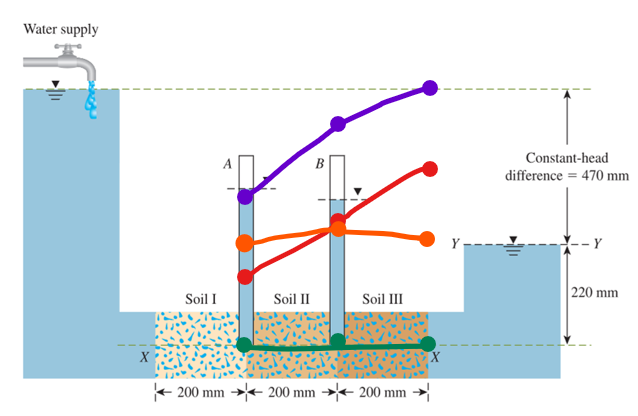
\includegraphics[scale=0.7, frame]{fig1.png}
    \\\emph{Figure 1: Cross Section for Initial $n$ Values of Station 5.99}\\
    \vspace{5mm}
    \addcontentsline{lof}{figure}{Figure 2: Cross Section for Halved $n$ Values of Station 5.99}
    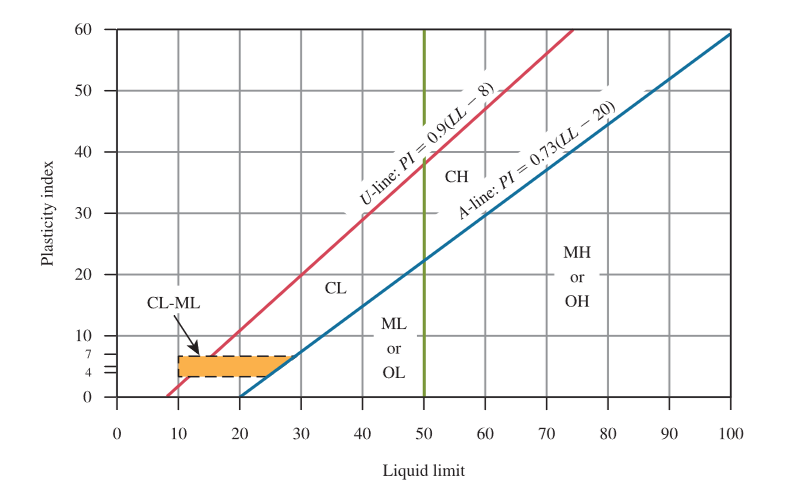
\includegraphics[scale=0.7, frame]{fig2.png}
    \\\emph{Figure 2: Cross Section for Halved $n$ Values of Station 5.99}\\
    \vspace{5mm}
    \addcontentsline{lof}{figure}{Figure 3: Cross Section for Doubled $n$ Values of Station 5.99}
    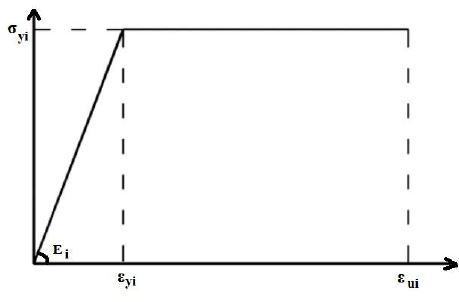
\includegraphics[scale=0.7, frame]{fig3.png}
    \\\emph{Figure 3: Cross Section for Doubled $n$ Values of Station 5.99}\\
\end{center}\newpage

%Station 5.76 Initial
\end{center}
\subsubsection{Station 5.76}
\begin{center}
\addcontentsline{lot}{table}{Table 7: Initial $n$ Values for Station 5.76}
\begin{tabular}{|cc||cc||cc|} 
    \hline
    \multicolumn{2}{|c||}{\textbf{Fill}} & \multicolumn{2}{c||}{\textbf{Ground}} & \multicolumn{2}{c|}{\textbf{Levee}}           \\ 
    \hline
    x        & y                        & x    & y                             & x        & y                                  \\
    58.79404 & 215.1951                 & 0    & 218.7                         & 906      & 214.3                              \\
    1549.358 & 215.1951                 & 16   & 218.1                         &          &                                    \\
    1486     & 214.2                    & 39   & 216.4                         & \multicolumn{2}{c|}{\textbf{Bank Station}}    \\ 
    \cline{5-6}
    1463     & 214                      & 85   & 213.6                         & x        & y                                  \\
    1440     & 214.5                    & 262  & 213                           & 351      & 214.4                              \\
    1362     & 213.6                    & 351  & 214.4                         & 548      & 212.7                              \\
    1332     & 209                      & 390  & 210.9                         &          &                                    \\
    1250     & 212                      & 404  & 206.4                         & \multicolumn{2}{c|}{\textbf{Water Surface}}   \\ 
    \cline{5-6}
    1240     & 211.8                    & 423  & 205                           & x        & y                                  \\
    1139     & 210.2                    & 446  & 211.7                         & 58.79404 & 215.1951                           \\
    1129     & 210.3                    & 459  & 211.5                         & 1549.358 & 215.1951                           \\
    1099     & 210.3                    & 472  & 210.1                         & 423      & 215.1951                           \\
    1099     & 209.5                    & 489  & 211.9                         &          &                                    \\
    1079     & 215                      & 541  & 212                           & \multicolumn{2}{c|}{\textbf{Energy Grade}}    \\ 
    \cline{5-6}
    1030     & 210.2                    & 548  & 212.7                         & x        & y                                  \\
    991      & 209.6                    & 666  & 213.9                         & 56.87808 & 215.3118                           \\
    981      & 209.2                    & 705  & 213.9                         & 1556.783 & 215.3118                           \\
    971      & 213.5                    & 715  & 213.9                         & 423      & 215.3118                           \\
    945      & 213.9                    & 728  & 213.9                         &          &                                    \\
    906      & 214.3                    & 755  & 213.9                         & \multicolumn{2}{c|}{\textbf{Critical Level}}  \\ 
    \cline{5-6}
    833      & 213.9                    & 791  & 213.9                         & x        & y                                  \\
    814      & 213.9                    & 814  & 213.9                         & 145.7765 & 213.394                            \\
    791      & 213.9                    & 833  & 213.9                         & 287.0461 & 213.394                            \\
    755      & 213.9                    & 906  & 214.3                         & 362.2098 & 213.394                            \\
    728      & 213.9                    & 945  & 213.9                         & 616.242  & 213.394                            \\
    715      & 213.9                    & 971  & 213.5                         & 423      & 213.394                            \\
    705      & 213.9                    & 981  & 209.2                         &          &                                    \\
    666      & 213.9                    & 991  & 209.6                         &          &                                    \\
    548      & 212.7                    & 1030 & 210.2                         &          &                                    \\
    541      & 212                      & 1079 & 215                           &          &                                    \\
    489      & 211.9                    & 1099 & 209.5                         &          &                                    \\
    472      & 210.1                    & 1099 & 210.3                         &          &                                    \\
    459      & 211.5                    & 1129 & 210.3                         &          &                                    \\
    446      & 211.7                    & 1139 & 210.2                         &          &                                    \\
    423      & 205                      & 1240 & 211.8                         &          &                                    \\
    404      & 206.4                    & 1250 & 212                           &          &                                    \\
    390      & 210.9                    & 1332 & 209                           &          &                                    \\
    351      & 214.4                    & 1362 & 213.6                         &          &                                    \\
    262      & 213                      & 1440 & 214.5                         &          &                                    \\
    85       & 213.6                    & 1463 & 214                           &          &                                    \\
             &                          & 1486 & 214.2                         &          &                                    \\
             &                          & 1677 & 217.2                         &          &                                    \\
             &                          & 1805 & 218.9                         &          &                                    \\
    \hline\multicolumn{6}{c}{\emph{Table 7: Initial $n$ Values for Station 5.76}}
\end{tabular}

%Station 5.76 Halved

\addcontentsline{lot}{table}{Table 8: Halved $n$ Values for Station 5.76}
\begin{tabular}{|cc||cc||cc|} 
    \hline
    \multicolumn{2}{|c||}{\textbf{Fill }} & \multicolumn{2}{c||}{\textbf{Ground }} & \multicolumn{2}{c|}{\textbf{Levee }}           \\ 
    \hline
    x        & y                         & x    & y                              & x        & y                                   \\
    83.36731 & 213.6994                  & 0    & 218.7                          & 906      & 214.3                               \\
    306.4612 & 213.6994                  & 16   & 218.1                          &          &                                     \\
    262      & 213                       & 39   & 216.4                          & \multicolumn{2}{c|}{\textbf{Bank Station }}    \\ 
    \cline{5-6}
    85       & 213.6                     & 85   & 213.6                          & x        & y                                   \\
    358.8068 & 213.6994                  & 262  & 213                            & 351      & 214.4                               \\
    646.2736 & 213.6994                  & 351  & 214.4                          & 548      & 212.7                               \\
    548      & 212.7                     & 390  & 210.9                          &          &                                     \\
    541      & 212                       & 404  & 206.4                          & \multicolumn{2}{c|}{\textbf{Water Surface }}   \\ 
    \cline{5-6}
    489      & 211.9                     & 423  & 205                            & x        & y                                   \\
    472      & 210.1                     & 446  & 211.7                          & 83.36731 & 213.6994                            \\
    459      & 211.5                     & 459  & 211.5                          & 306.4612 & 213.6994                            \\
    446      & 211.7                     & 472  & 210.1                          & 358.8068 & 213.6994                            \\
    423      & 205                       & 489  & 211.9                          & 646.2736 & 213.6994                            \\
    404      & 206.4                     & 541  & 212                            & 423      & 213.6994                            \\
    390      & 210.9                     & 548  & 212.7                          &          &                                     \\
             &                           & 666  & 213.9                          & \multicolumn{2}{c|}{\textbf{Energy Grade }}    \\ 
    \cline{5-6}
             &                           & 705  & 213.9                          & x        & y                                   \\
             &                           & 715  & 213.9                          & 66.74715 & 214.711                             \\
             &                           & 728  & 213.9                          & 1076.05  & 214.711                             \\
             &                           & 755  & 213.9                          & 1080.051 & 214.711                             \\
             &                           & 791  & 213.9                          & 1518.537 & 214.711                             \\
             &                           & 814  & 213.9                          & 423      & 214.711                             \\
             &                           & 833  & 213.9                          &          &                                     \\
             &                           & 906  & 214.3                          & \multicolumn{2}{c|}{\textbf{Critical Level }}  \\ 
    \cline{5-6}
             &                           & 945  & 213.9                          & x        & y                                   \\
             &                           & 971  & 213.5                          & 145.7765 & 213.394                             \\
             &                           & 981  & 209.2                          & 287.0461 & 213.394                             \\
             &                           & 991  & 209.6                          & 362.2098 & 213.394                             \\
             &                           & 1030 & 210.2                          & 616.242  & 213.394                             \\
             &                           & 1079 & 215                            & 423      & 213.394                             \\
             &                           & 1099 & 209.5                          &          &                                     \\
             &                           & 1099 & 210.3                          &          &                                     \\
             &                           & 1129 & 210.3                          &          &                                     \\
             &                           & 1139 & 210.2                          &          &                                     \\
             &                           & 1240 & 211.8                          &          &                                     \\
             &                           & 1250 & 212                            &          &                                     \\
             &                           & 1332 & 209                            &          &                                     \\
             &                           & 1362 & 213.6                          &          &                                     \\
             &                           & 1440 & 214.5                          &          &                                     \\
             &                           & 1463 & 214                            &          &                                     \\
             &                           & 1486 & 214.2                          &          &                                     \\
             &                           & 1677 & 217.2                          &          &                                     \\
             &                           & 1805 & 218.9                          &          &                                     \\
    \hline\multicolumn{6}{c}{\emph{Table 8: Halved $n$ Values for Station 5.76}}
\end{tabular}

%5.76 Doubled

\addcontentsline{lot}{table}{Table 9: Doubled $n$ Values for Station 5.76}
\begin{tabular}{|cc||cc||cc|} 
    \hline
    \multicolumn{2}{|c||}{\textbf{Fill }} & \multicolumn{2}{c||}{\textbf{Ground }} & \multicolumn{2}{c|}{\textbf{Levee }}           \\ 
    \hline
    x        & y                         & x    & y                              & x        & y                                   \\
    33.782   & 216.7857                  & 0    & 218.7                          & 906      & 214.3                               \\
    1650.621 & 216.7857                  & 16   & 218.1                          &          &                                     \\
    1486     & 214.2                     & 39   & 216.4                          & \multicolumn{2}{c|}{\textbf{Bank Station }}    \\ 
    \cline{5-6}
    1463     & 214                       & 85   & 213.6                          & x        & y                                   \\
    1440     & 214.5                     & 262  & 213                            & 351      & 214.4                               \\
    1362     & 213.6                     & 351  & 214.4                          & 548      & 212.7                               \\
    1332     & 209                       & 390  & 210.9                          &          &                                     \\
    1250     & 212                       & 404  & 206.4                          & \multicolumn{2}{c|}{\textbf{Water Surface }}   \\ 
    \cline{5-6}
    1240     & 211.8                     & 423  & 205                            & x        & y                                   \\
    1139     & 210.2                     & 446  & 211.7                          & 33.782   & 216.7857                            \\
    1129     & 210.3                     & 459  & 211.5                          & 1650.621 & 216.7857                            \\
    1099     & 210.3                     & 472  & 210.1                          & 423      & 216.7857                            \\
    1099     & 209.5                     & 489  & 211.9                          &          &                                     \\
    1079     & 215                       & 541  & 212                            & \multicolumn{2}{c|}{\textbf{Energy Grade }}    \\ 
    \cline{5-6}
    1030     & 210.2                     & 548  & 212.7                          & x        & y                                   \\
    991      & 209.6                     & 666  & 213.9                          & 33.23431 & 216.8262                            \\
    981      & 209.2                     & 705  & 213.9                          & 1653.199 & 216.8262                            \\
    971      & 213.5                     & 715  & 213.9                          & 423      & 216.8262                            \\
    945      & 213.9                     & 728  & 213.9                          &          &                                     \\
    906      & 214.3                     & 755  & 213.9                          & \multicolumn{2}{c|}{\textbf{Critical Level }}  \\ 
    \cline{5-6}
    833      & 213.9                     & 791  & 213.9                          & x        & y                                   \\
    814      & 213.9                     & 814  & 213.9                          & 145.7765 & 213.394                             \\
    791      & 213.9                     & 833  & 213.9                          & 287.0461 & 213.394                             \\
    755      & 213.9                     & 906  & 214.3                          & 362.2098 & 213.394                             \\
    728      & 213.9                     & 945  & 213.9                          & 616.242  & 213.394                             \\
    715      & 213.9                     & 971  & 213.5                          & 423      & 213.394                             \\
    705      & 213.9                     & 981  & 209.2                          &          &                                     \\
    666      & 213.9                     & 991  & 209.6                          &          &                                     \\
    548      & 212.7                     & 1030 & 210.2                          &          &                                     \\
    541      & 212                       & 1079 & 215                            &          &                                     \\
    489      & 211.9                     & 1099 & 209.5                          &          &                                     \\
    472      & 210.1                     & 1099 & 210.3                          &          &                                     \\
    459      & 211.5                     & 1129 & 210.3                          &          &                                     \\
    446      & 211.7                     & 1139 & 210.2                          &          &                                     \\
    423      & 205                       & 1240 & 211.8                          &          &                                     \\
    404      & 206.4                     & 1250 & 212                            &          &                                     \\
    390      & 210.9                     & 1332 & 209                            &          &                                     \\
    351      & 214.4                     & 1362 & 213.6                          &          &                                     \\
    262      & 213                       & 1440 & 214.5                          &          &                                     \\
    85       & 213.6                     & 1463 & 214                            &          &                                     \\
    39       & 216.4                     & 1486 & 214.2                          &          &                                     \\
    0        & 218.7                     & 1677 & 217.2                          &          &                                     \\
             &                           & 1805 & 218.9                          &          &                                     \\
    \hline\multicolumn{6}{c}{\emph{Table 9: Doubled $n$ Values for Station 5.76}}
\end{tabular}

\newpage\begin{center}
    \addcontentsline{lof}{figure}{Figure 4: Cross Section for Initial $n$ Values of Station 5.76}
    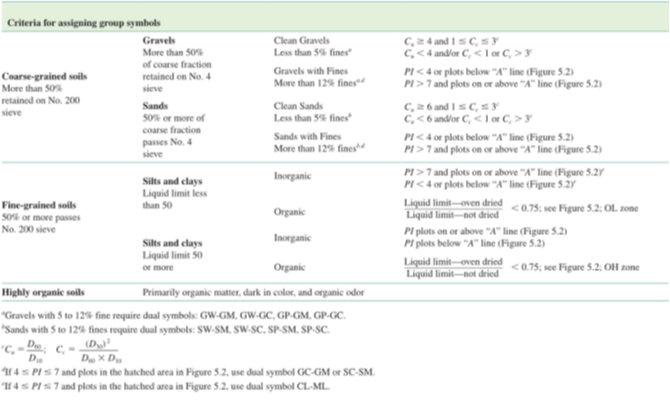
\includegraphics[scale=0.7, frame]{fig4.png}
    \\\emph{Figure 4: Cross Section for Initial $n$ Values of Station 5.76}\\
    \vspace{5mm}
    \addcontentsline{lof}{figure}{Figure 5: Cross Section for Halved $n$ Values of Station 5.76}
    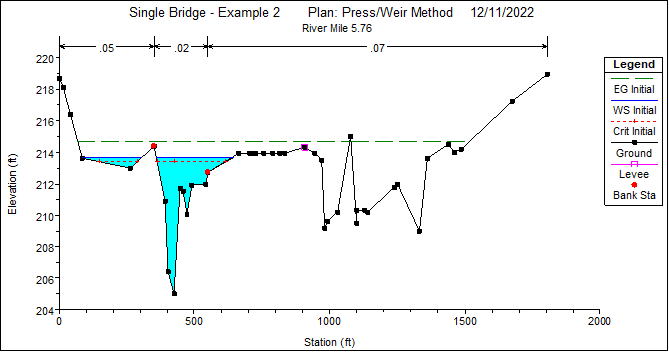
\includegraphics[scale=0.7, frame]{fig5.png}
    \\\emph{Figure 5: Cross Section for Halved $n$ Values of Station 5.76}\\
    \vspace{5mm}
    \addcontentsline{lof}{figure}{Figure 6: Cross Section for Doubled $n$ Values of Station 5.76}
    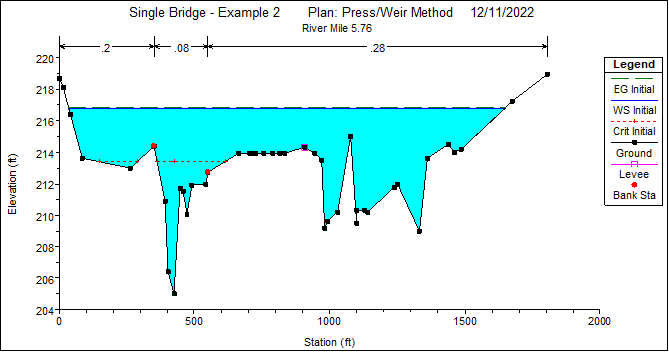
\includegraphics[scale=0.7, frame]{fig6.png}
    \\\emph{Figure 6: Cross Section for Doubled $n$ Values of Station 5.76}\\
\end{center}\newpage


\end{center}
\subsubsection{Station 5.39}
\begin{center}
% Station 5.39 Initial
\addcontentsline{lot}{table}{Table 10: Initial $n$ Values for Station 5.39}
\begin{tabular}{|cccc||cccc||cc|} 
    \hline
    \multicolumn{2}{|c}{\textbf{Fill }} & \multicolumn{2}{c||}{\textbf{Ground }} & \multicolumn{2}{c}{\textbf{Fill (cont'd)}} & \multicolumn{2}{c||}{\textbf{Ground (cont'd)}} & \multicolumn{2}{c|}{\textbf{Inefficiency }}    \\ 
    \hline
    x        & y                        & x     & y                             & x        & y                       & x     & y                             & x        & y                                   \\
    132.172  & 212.7437                 & 0     & 216.8                         & 668.2709 & 212.7437                & 643.6 & 213.1                         & 420      & 211.1329                            \\
    448.233  & 212.7437                 & 89    & 213.6                         & 815.742  & 212.7437                & 647   & 213.5                         & 420      & 215                                 \\
    443      & 210.8                    & 210   & 211.2                         & 692      & 211.9                   & 692   & 211.9                         & 677      & 212.4333                            \\
    367      & 211.9                    & 285   & 210.8                         & 991.0397 & 212.7437                & 824   & 212.8                         & 677      & 215                                 \\
    285      & 210.8                    & 367   & 211.9                         & 1463.4   & 212.7437                & 896   & 213.3                         &          &                                     \\
    210      & 211.2                    & 443   & 210.8                         & 1421     & 211.7                   & 961   & 213.2                         & \multicolumn{2}{c|}{\textbf{Bank Station }}    \\ 
    \cline{9-10}
    456.9847 & 212.7437                 & 450   & 213.4                         & 1371     & 211.5                   & 1040  & 212                           & x        & y                                   \\
    642.2935 & 212.7437                 & 456.6 & 212.9                         & 1309     & 210.2                   & 1093  & 211.7                         & 450      & 213.4                               \\
    640.3    & 212.2                    & 459.8 & 211.6                         & 1243     & 211.1                   & 1116  & 210                           & 647      & 213.5                               \\
    633.7    & 211.3                    & 466.4 & 210.1                         & 1116     & 210                     & 1243  & 211.1                         &          &                                     \\
    630.5    & 209.6                    & 469.7 & 209.3                         & 1093     & 211.7                   & 1309  & 210.2                         & \multicolumn{2}{c|}{\textbf{Water Surface }}   \\ 
    \cline{9-10}
    623.9    & 209.3                    & 476.2 & 208.9                         & 1040     & 212                     & 1371  & 211.5                         & x        & y                                   \\
    620.6    & 209                      & 479.5 & 208.6                         &          &                         & 1421  & 211.7                         & 132.172  & 212.7437                            \\
    614.1    & 208.7                    & 486.1 & 208.7                         &          &                         & 1486  & 213.3                         & 448.233  & 212.7437                            \\
    610.8    & 208                      & 489.4 & 207.9                         &          &                         & 1558  & 213.7                         & 456.9847 & 212.7437                            \\
    604.2    & 207.5                    & 495.9 & 208.8                         &          &                         & 1660  & 214.7                         & 642.2935 & 212.7437                            \\
    600.9    & 206.5                    & 499.2 & 208.6                         &          &                         & 1723  & 215.4                         & 668.2709 & 212.7437                            \\
    594.4    & 205.8                    & 505.8 & 207.8                         &          &                         & 1824  & 217.1                         & 815.742  & 212.7437                            \\
    591.1    & 204.7                    & 509.1 & 207.6                         &          &                         &       &                               & 991.0397 & 212.7437                            \\
    584.5    & 204                      & 515.6 & 206.9                         &          &                         &       &                               & 1463.4   & 212.7437                            \\
    581.2    & 203.6                    & 518.9 & 204.3                         &          &                         &       &                               & 548.4    & 212.7437                            \\
    574.7    & 202.9                    & 525.5 & 203.6                         &          &                         &       &                               &          &                                     \\
    571.4    & 203                      & 528.7 & 203.4                         &          &                         &       &                               & \multicolumn{2}{c|}{\textbf{Energy Grade }}    \\ 
    \cline{9-10}
    564.8    & 203.8                    & 535.3 & 203.1                         &          &                         &       &                               & x        & y                                   \\
    561.6    & 204.4                    & 538.6 & 202.9                         &          &                         &       &                               & 116.9662 & 213.0453                            \\
    555      & 203.1                    & 545.1 & 203                           &          &                         &       &                               & 449.0451 & 213.0453                            \\
    548.4    & 202.7                    & 548.4 & 202.7                         &          &                         &       &                               & 454.6819 & 213.0453                            \\
    545.1    & 203                      & 555   & 203.1                         &          &                         &       &                               & 643.3994 & 213.0453                            \\
    538.6    & 202.9                    & 561.6 & 204.4                         &          &                         &       &                               & 659.7883 & 213.0453                            \\
    535.3    & 203.1                    & 564.8 & 203.8                         &          &                         &       &                               & 859.3232 & 213.0453                            \\
    528.7    & 203.4                    & 571.4 & 203                           &          &                         &       &                               & 971.184  & 213.0453                            \\
    525.5    & 203.6                    & 574.7 & 202.9                         &          &                         &       &                               & 1475.653 & 213.0453                            \\
    518.9    & 204.3                    & 581.2 & 203.6                         &          &                         &       &                               & 548.4    & 213.0453                            \\
    515.6    & 206.9                    & 584.5 & 204                           &          &                         &       &                               &          &                                     \\
    509.1    & 207.6                    & 591.1 & 204.7                         &          &                         &       &                               & \multicolumn{2}{c|}{\textbf{Critical Level }}  \\ 
    \cline{9-10}
    505.8    & 207.8                    & 594.4 & 205.8                         &          &                         &       &                               & x        & y                                   \\
    499.2    & 208.6                    & 600.9 & 206.5                         &          &                         &       &                               & 476.0116 & 208.9116                            \\
    495.9    & 208.8                    & 604.2 & 207.5                         &          &                         &       &                               & 618.6844 & 208.9116                            \\
    489.4    & 207.9                    & 610.8 & 208                           &          &                         &       &                               & 548.4    & 208.9116                            \\
    486.1    & 208.7                    & 614.1 & 208.7                         &          &                         &       &                               &          &                                     \\
    479.5    & 208.6                    & 620.6 & 209                           &          &                         &       &                               &          &                                     \\
    476.2    & 208.9                    & 623.9 & 209.3                         &          &                         &       &                               &          &                                     \\
    469.7    & 209.3                    & 630.5 & 209.6                         &          &                         &       &                               &          &                                     \\
    466.4    & 210.1                    & 633.7 & 211.3                         &          &                         &       &                               &          &                                     \\
    459.8    & 211.6                    & 640.3 & 212.2                         &          &                         &       &                               &          &                                     \\
    \hline\multicolumn{10}{c}{\emph{Table 10: Initial $n$ Values for Station 5.39}}
\end{tabular}

% Station 5.39 Halved
\addcontentsline{lot}{table}{Table 11: Halved $n$ Values for Station 5.39}
\begin{tabular}{|cccc||cccc||cc|} 
    \hline
    \multicolumn{2}{|c}{\textbf{Fill}} & \multicolumn{2}{c||}{\textbf{Ground}} & \multicolumn{2}{c}{\textbf{Fill (cont'd)}} & \multicolumn{2}{c||}{\textbf{Ground (cont'd)}} & \multicolumn{2}{c|}{\textbf{Inefficiency}}    \\ 
    \hline
    x        & y                       & x     & y                            & x        & y                      & x     & y                            & x        & y                                  \\
    194.9203 & 211.4991                & 0     & 216.8                        & 476.2    & 208.9                  & 623.9 & 209.3                        & 420      & 211.1329                           \\
    337.1149 & 211.4991                & 89    & 213.6                        & 469.7    & 209.3                  & 630.5 & 209.6                        & 420      & 215                                \\
    285      & 210.8                   & 210   & 211.2                        & 466.4    & 210.1                  & 633.7 & 211.3                        & 677      & 212.4333                           \\
    210      & 211.2                   & 285   & 210.8                        & 1095.718 & 211.4991               & 640.3 & 212.2                        & 677      & 215                                \\
    394.6984 & 211.4991                & 367   & 211.9                        & 1370.957 & 211.4991               & 643.6 & 213.1                        &          &                                    \\
    444.8822 & 211.4991                & 443   & 210.8                        & 1309     & 210.2                  & 647   & 213.5                        & \multicolumn{2}{c|}{\textbf{Bank Station}}    \\ 
    \cline{9-10}
    443      & 210.8                   & 450   & 213.4                        & 1243     & 211.1                  & 692   & 211.9                        & x        & y                                  \\
    460.244  & 211.4991                & 456.6 & 212.9                        & 1116     & 210                    & 824   & 212.8                        & 450      & 213.4                              \\
    635.16   & 211.4991                & 459.8 & 211.6                        &          &                        & 896   & 213.3                        & 647      & 213.5                              \\
    633.7    & 211.3                   & 466.4 & 210.1                        &          &                        & 961   & 213.2                        &          &                                    \\
    630.5    & 209.6                   & 469.7 & 209.3                        &          &                        & 1040  & 212                          & \multicolumn{2}{c|}{\textbf{Water Surface}}   \\ 
    \cline{9-10}
    623.9    & 209.3                   & 476.2 & 208.9                        &          &                        & 1093  & 211.7                        & x        & y                                  \\
    620.6    & 209                     & 479.5 & 208.6                        &          &                        & 1116  & 210                          & 194.9203 & 211.4991                           \\
    614.1    & 208.7                   & 486.1 & 208.7                        &          &                        & 1243  & 211.1                        & 337.1149 & 211.4991                           \\
    610.8    & 208                     & 489.4 & 207.9                        &          &                        & 1309  & 210.2                        & 394.6984 & 211.4991                           \\
    604.2    & 207.5                   & 495.9 & 208.8                        &          &                        & 1371  & 211.5                        & 444.8822 & 211.4991                           \\
    600.9    & 206.5                   & 499.2 & 208.6                        &          &                        & 1421  & 211.7                        & 460.244  & 211.4991                           \\
    594.4    & 205.8                   & 505.8 & 207.8                        &          &                        & 1486  & 213.3                        & 635.16   & 211.4991                           \\
    591.1    & 204.7                   & 509.1 & 207.6                        &          &                        & 1558  & 213.7                        & 1095.718 & 211.4991                           \\
    584.5    & 204                     & 515.6 & 206.9                        &          &                        & 1660  & 214.7                        & 1370.957 & 211.4991                           \\
    581.2    & 203.6                   & 518.9 & 204.3                        &          &                        & 1723  & 215.4                        & 548.4    & 211.4991                           \\
    574.7    & 202.9                   & 525.5 & 203.6                        &          &                        & 1824  & 217.1                        &          &                                    \\
    571.4    & 203                     & 528.7 & 203.4                        &          &                        &       &                              & \multicolumn{2}{c|}{\textbf{Energy Grade}}    \\ 
    \cline{9-10}
    564.8    & 203.8                   & 535.3 & 203.1                        &          &                        &       &                              & x        & y                                  \\
    561.6    & 204.4                   & 538.6 & 202.9                        &          &                        &       &                              & 171.0083 & 211.9734                           \\
    555      & 203.1                   & 545.1 & 203                          &          &                        &       &                              & 446.1591 & 211.9734                           \\
    548.4    & 202.7                   & 548.4 & 202.7                        &          &                        &       &                              & 458.8809 & 211.9734                           \\
    545.1    & 203                     & 555   & 203.1                        &          &                        &       &                              & 638.6382 & 211.9734                           \\
    538.6    & 202.9                   & 561.6 & 204.4                        &          &                        &       &                              & 689.9358 & 211.9734                           \\
    535.3    & 203.1                   & 564.8 & 203.8                        &          &                        &       &                              & 702.7645 & 211.9734                           \\
    528.7    & 203.4                   & 571.4 & 203                          &          &                        &       &                              & 1044.701 & 211.9734                           \\
    525.5    & 203.6                   & 574.7 & 202.9                        &          &                        &       &                              & 1432.106 & 211.9734                           \\
    518.9    & 204.3                   & 581.2 & 203.6                        &          &                        &       &                              & 548.4    & 211.9734                           \\
    515.6    & 206.9                   & 584.5 & 204                          &          &                        &       &                              &          &                                    \\
    509.1    & 207.6                   & 591.1 & 204.7                        &          &                        &       &                              & \multicolumn{2}{c|}{\textbf{Critical Level}}  \\ 
    \cline{9-10}
    505.8    & 207.8                   & 594.4 & 205.8                        &          &                        &       &                              & x        & y                                  \\
    499.2    & 208.6                   & 600.9 & 206.5                        &          &                        &       &                              & 476.0116 & 208.9116                           \\
    495.9    & 208.8                   & 604.2 & 207.5                        &          &                        &       &                              & 618.6844 & 208.9116                           \\
    489.4    & 207.9                   & 610.8 & 208                          &          &                        &       &                              & 548.4    & 208.9116                           \\
    486.1    & 208.7                   & 614.1 & 208.7                        &          &                        &       &                              &          &                                    \\
    479.5    & 208.6                   & 620.6 & 209                          &          &                        &       &                              &          &                                    \\
    476.2    & 208.9                   & 623.9 & 209.3                        &          &                        &       &                              &          &                                    \\
    469.7    & 209.3                   & 630.5 & 209.6                        &          &                        &       &                              &          &                                    \\
    466.4    & 210.1                   & 633.7 & 211.3                        &          &                        &       &                              &          &                                    \\
    459.8    & 211.6                   & 640.3 & 212.2                        &          &                        &       &                              &          &                                    \\
    \hline\multicolumn{10}{c}{\emph{Table 11: Halved $n$ Values for Station 5.39}}
\end{tabular}

% Station 5.39 Doubled
\addcontentsline{lot}{table}{Table 12: Doubled $n$ Values for Station 5.39}
\begin{tabular}{|cccc||cccc||cc|} 
    \hline
    \multicolumn{2}{|c}{\textbf{Fill}} & \multicolumn{2}{c||}{\textbf{Ground}} & \multicolumn{2}{c}{\textbf{Fill (cont'd)}} & \multicolumn{2}{c||}{\textbf{Ground (cont'd)}} & \multicolumn{2}{c|}{\textbf{Inefficiency}}    \\ 
    \hline
    x        & y                       & x     & y                            & x     & y                         & x     & y                            & x        & y                                  \\
    63.71426 & 214.5092                & 0     & 216.8                        & 561.6 & 204.4                     & 584.5 & 204                          & 420      & 211.1329                           \\
    1640.534 & 214.5092                & 89    & 213.6                        & 555   & 203.1                     & 591.1 & 204.7                        & 420      & 215                                \\
    1558     & 213.7                   & 210   & 211.2                        & 548.4 & 202.7                     & 594.4 & 205.8                        & 677      & 212.4333                           \\
    1486     & 213.3                   & 285   & 210.8                        & 545.1 & 203                       & 600.9 & 206.5                        & 677      & 215                                \\
    1421     & 211.7                   & 367   & 211.9                        & 538.6 & 202.9                     & 604.2 & 207.5                        &          &                                    \\
    1371     & 211.5                   & 443   & 210.8                        & 535.3 & 203.1                     & 610.8 & 208                          & \multicolumn{2}{c|}{\textbf{Bank Station}}    \\ 
    \cline{9-10}
    1309     & 210.2                   & 450   & 213.4                        & 528.7 & 203.4                     & 614.1 & 208.7                        & x        & y                                  \\
    1243     & 211.1                   & 456.6 & 212.9                        & 525.5 & 203.6                     & 620.6 & 209                          & 450      & 213.4                              \\
    1116     & 210                     & 459.8 & 211.6                        & 518.9 & 204.3                     & 623.9 & 209.3                        & 647      & 213.5                              \\
    1093     & 211.7                   & 466.4 & 210.1                        & 515.6 & 206.9                     & 630.5 & 209.6                        &          &                                    \\
    1040     & 212                     & 469.7 & 209.3                        & 509.1 & 207.6                     & 633.7 & 211.3                        & \multicolumn{2}{c|}{\textbf{Water Surface}}   \\ 
    \cline{9-10}
    961      & 213.2                   & 476.2 & 208.9                        & 505.8 & 207.8                     & 640.3 & 212.2                        & x        & y                                  \\
    896      & 213.3                   & 479.5 & 208.6                        & 499.2 & 208.6                     & 643.6 & 213.1                        & 63.71426 & 214.5092                           \\
    824      & 212.8                   & 486.1 & 208.7                        & 495.9 & 208.8                     & 647   & 213.5                        & 1640.534 & 214.5092                           \\
    692      & 211.9                   & 489.4 & 207.9                        & 489.4 & 207.9                     & 692   & 211.9                        & 548.4    & 214.5092                           \\
    647      & 213.5                   & 495.9 & 208.8                        & 486.1 & 208.7                     & 824   & 212.8                        &          &                                    \\
    643.6    & 213.1                   & 499.2 & 208.6                        & 479.5 & 208.6                     & 896   & 213.3                        & \multicolumn{2}{c|}{\textbf{Energy Grade }}   \\ 
    \cline{9-10}
    640.3    & 212.2                   & 505.8 & 207.8                        & 476.2 & 208.9                     & 961   & 213.2                        & x        & y                                  \\
    633.7    & 211.3                   & 509.1 & 207.6                        & 469.7 & 209.3                     & 1040  & 212                          & 58.87372 & 214.6832                           \\
    630.5    & 209.6                   & 515.6 & 206.9                        & 466.4 & 210.1                     & 1093  & 211.7                        & 1658.286 & 214.6832                           \\
    623.9    & 209.3                   & 518.9 & 204.3                        & 459.8 & 211.6                     & 1116  & 210                          & 548.4    & 214.6832                           \\
    620.6    & 209                     & 525.5 & 203.6                        & 456.6 & 212.9                     & 1243  & 211.1                        &          &                                    \\
    614.1    & 208.7                   & 528.7 & 203.4                        & 450   & 213.4                     & 1309  & 210.2                        & \multicolumn{2}{c|}{\textbf{Critical Level}}  \\ 
    \cline{9-10}
    610.8    & 208                     & 535.3 & 203.1                        & 443   & 210.8                     & 1371  & 211.5                        & x        & y                                  \\
    604.2    & 207.5                   & 538.6 & 202.9                        & 367   & 211.9                     & 1421  & 211.7                        & 476.0116 & 208.9116                           \\
    600.9    & 206.5                   & 545.1 & 203                          & 285   & 210.8                     & 1486  & 213.3                        & 618.6844 & 208.9116                           \\
    594.4    & 205.8                   & 548.4 & 202.7                        & 210   & 211.2                     & 1558  & 213.7                        & 548.4    & 208.9116                           \\
    591.1    & 204.7                   & 555   & 203.1                        & 89    & 213.6                     & 1660  & 214.7                        &          &                                    \\
    584.5    & 204                     & 561.6 & 204.4                        & 0     & 216.8                     & 1723  & 215.4                        &          &                                    \\
    581.2    & 203.6                   & 564.8 & 203.8                        &       &                           & 1824  & 217.1                        &          &                                    \\
    574.7    & 202.9                   & 571.4 & 203                          &       &                           &       &                              &          &                                    \\
    571.4    & 203                     & 574.7 & 202.9                        &       &                           &       &                              &          &                                    \\
    564.8    & 203.8                   & 581.2 & 203.6                        &       &                           &       &                              &          &                                    \\
    515.6    & 206.9                   & 584.5 & 204                          &       &                           &       &                              &          &                                    \\
    509.1    & 207.6                   & 591.1 & 204.7                        &       &                           &       &                              &          & \multicolumn{1}{l|}{}              \\
    505.8    & 207.8                   & 594.4 & 205.8                        &       &                           &       &                              &          &                                    \\
    499.2    & 208.6                   & 600.9 & 206.5                        &       &                           &       &                              &          &                                    \\
    495.9    & 208.8                   & 604.2 & 207.5                        &       &                           &       &                              &          &                                    \\
    489.4    & 207.9                   & 610.8 & 208                          &       &                           &       &                              &          &                                    \\
    486.1    & 208.7                   & 614.1 & 208.7                        &       &                           &       &                              &          &                                    \\
    479.5    & 208.6                   & 620.6 & 209                          &       &                           &       &                              &          &                                    \\
    476.2    & 208.9                   & 623.9 & 209.3                        &       &                           &       &                              &          &                                    \\
    469.7    & 209.3                   & 630.5 & 209.6                        &       &                           &       &                              &          &                                    \\
    466.4    & 210.1                   & 633.7 & 211.3                        &       &                           &       &                              &          &                                    \\
    459.8    & 211.6                   & 640.3 & 212.2                        &       &                           &       &                              &          &                                    \\
    \hline\multicolumn{10}{c}{\emph{Table 12: Doubled $n$ Values for Station 5.39}}
\end{tabular}


\newpage\begin{center}
    \addcontentsline{lof}{figure}{Figure 7: Cross Section for Initial $n$ Values of Station 5.39}
    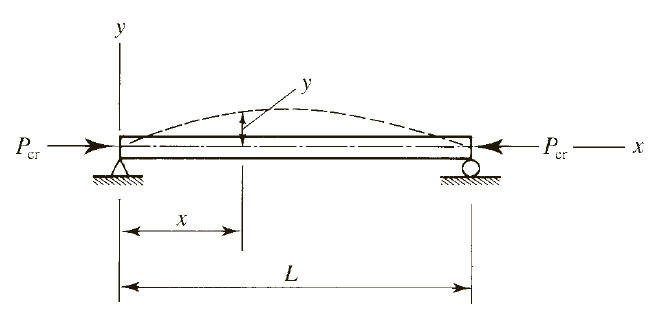
\includegraphics[scale=0.7, frame]{fig7.png}
    \\\emph{Figure 7: Cross Section for Initial $n$ Values of Station 5.39}\\
    \vspace{5mm}
    \addcontentsline{lof}{figure}{Figure 8: Cross Section for Halved $n$ Values of Station 5.39}
    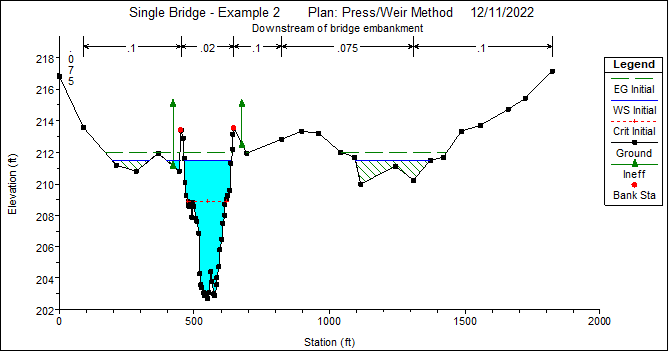
\includegraphics[scale=0.7, frame]{fig8.png}
    \\\emph{Figure 8: Cross Section for Halved $n$ Values of Station 5.39}\\
    \vspace{5mm}
    \addcontentsline{lof}{figure}{Figure 9: Cross Section for Doubled $n$ Values of Station 5.39}
    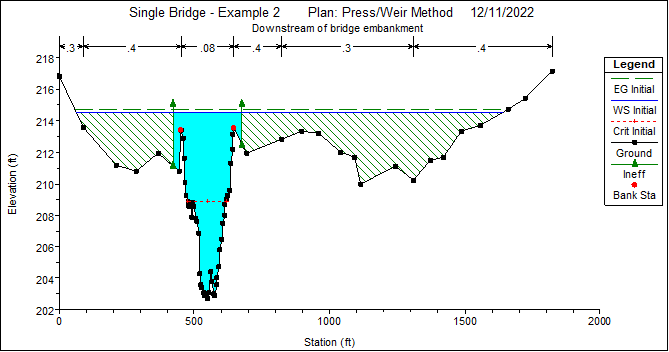
\includegraphics[scale=0.7, frame]{fig9.png}
    \\\emph{Figure 9: Cross Section for Doubled $n$ Values of Station 5.39}\\
\end{center}\newpage

%Station 5.21 Initial

\end{center}
\subsubsection{Station 5.21}
\begin{center}

\addcontentsline{lot}{table}{Table 13: Initial $n$ Values for Station 5.21}
\begin{tabular}{|cccc||cc||cc|} 
    \hline
    \multicolumn{2}{|c}{\textbf{Fill }} & \multicolumn{2}{c||}{\textbf{Ground }} & \multicolumn{2}{c||}{\textbf{Ground (cont'd)}} & \multicolumn{2}{c|}{\textbf{Levee }}           \\ 
    \hline
    x        & y                        & x     & y                             & x      & y                            & x        & y                                   \\
    55.56815 & 211.7428                 & 0     & 216.15                        & 974.7  & 211.83                       & 383.6    & 209.29                              \\
    972.1729 & 211.7428                 & 5.9   & 215.41                        & 996.6  & 212.38                       &          &                                     \\
    946.3    & 210.85                   & 83.1  & 209.71                        & 1015.4 & 212.64                       & \multicolumn{2}{c|}{\textbf{Bank Station }}    \\ 
    \cline{7-8}
    943.4    & 210.72                   & 119.5 & 208.57                        & 1033.4 & 213.23                       & x        & y                                   \\
    933      & 210.59                   & 136.5 & 207.39                        & 1220.5 & 213.69                       & 189      & 206.95                              \\
    852.7    & 209.78                   & 161   & 206.62                        & 1296.6 & 213.87                       & 246      & 208.95                              \\
    782.9    & 207.83                   & 167   & 207.34                        & 1332.5 & 213.95                       &          &                                     \\
    776.6    & 208.32                   & 189   & 206.95                        & 1466.8 & 213.78                       & \multicolumn{2}{c|}{\textbf{Water Surface }}   \\ 
    \cline{7-8}
    758.6    & 209.3                    & 211.7 & 205.71                        & 1526.1 & 213.77                       & x        & y                                   \\
    688.2    & 209.73                   & 221.4 & 204.77                        & 1640.1 & 214.08                       & 55.56815 & 211.7428                            \\
    665.6    & 209.84                   & 227.5 & 203.79                        & 1650.4 & 214.19                       & 972.1729 & 211.7428                            \\
    598      & 209.34                   & 227.5 & 202.24                        & 1740.5 & 215.7                        & 231.5    & 211.7428                            \\
    589.5    & 209.1                    & 231.5 & 201.35                        &        &                              &          &                                     \\
    542.1    & 207.85                   & 236.9 & 204.06                        &        &                              & \multicolumn{2}{c|}{\textbf{Energy Grade }}    \\ 
    \cline{7-8}
    525.9    & 207.1                    & 236.9 & 206.01                        &        &                              & x        & y                                   \\
    513.6    & 207.41                   & 238.2 & 206.57                        &        &                              & 53.87888 & 211.8675                            \\
    461.4    & 208.1                    & 246   & 208.95                        &        &                              & 976.194  & 211.8675                            \\
    460.6    & 208.01                   & 292.5 & 208.94                        &        &                              & 231.5    & 211.8675                            \\
    451.9    & 207.13                   & 297.8 & 208.67                        &        &                              &          &                                     \\
    442.4    & 207.17                   & 308.6 & 208.24                        &        &                              & \multicolumn{2}{c|}{\textbf{Critical Level }}  \\ 
    \cline{7-8}
    435.8    & 207.29                   & 327.6 & 209.01                        &        &                              & x        & y                                   \\
    427.2    & 208.22                   & 339   & 209.06                        &        &                              & 77.36282 & 210.1336                            \\
    419.3    & 208.41                   & 379.8 & 209.23                        &        &                              & 887.7552 & 210.1336                            \\
    402.4    & 208.96                   & 383.6 & 209.29                        &        &                              & 231.5    & 210.1336                            \\
    383.6    & 209.29                   & 402.4 & 208.96                        &        &                              &          &                                     \\
    379.8    & 209.23                   & 419.3 & 208.41                        &        &                              &          &                                     \\
    339      & 209.06                   & 427.2 & 208.22                        &        &                              &          &                                     \\
    327.6    & 209.01                   & 435.8 & 207.29                        &        &                              &          &                                     \\
    308.6    & 208.24                   & 442.4 & 207.17                        &        &                              &          &                                     \\
    297.8    & 208.67                   & 451.9 & 207.13                        &        &                              &          &                                     \\
    292.5    & 208.94                   & 460.6 & 208.01                        &        &                              &          &                                     \\
    246      & 208.95                   & 461.4 & 208.1                         &        &                              &          &                                     \\
    238.2    & 206.57                   & 513.6 & 207.41                        &        &                              &          &                                     \\
    236.9    & 206.01                   & 525.9 & 207.1                         &        &                              &          &                                     \\
    236.9    & 204.06                   & 542.1 & 207.85                        &        &                              &          &                                     \\
    231.5    & 201.35                   & 589.5 & 209.1                         &        &                              &          &                                     \\
    227.5    & 202.24                   & 598   & 209.34                        &        &                              &          &                                     \\
    227.5    & 203.79                   & 665.6 & 209.84                        &        &                              &          &                                     \\
    221.4    & 204.77                   & 688.2 & 209.73                        &        &                              &          &                                     \\
    211.7    & 205.71                   & 758.6 & 209.3                         &        &                              &          &                                     \\
    189      & 206.95                   & 776.6 & 208.32                        &        &                              &          &                                     \\
    167      & 207.34                   & 782.9 & 207.83                        &        &                              &          &                                     \\
    161      & 206.62                   & 852.7 & 209.78                        &        &                              &          &                                     \\
    136.5    & 207.39                   & 933   & 210.59                        &        &                              &          &                                     \\
    119.5    & 208.57                   & 943.4 & 210.72                        &        &                              &          &                                     \\
    83.1     & 209.71                   & 946.3 & 210.85                        &        &                              &          &                                     \\
    \hline\multicolumn{8}{c}{\emph{Table 13: Initial $n$ Values for Station 5.21}}
\end{tabular}

% Station 5.21 Halved

\addcontentsline{lot}{table}{Table 14: Halved $n$ Values for Station 5.21}
\begin{tabular}{|cccc||cc||cc|} 
    \hline
    \multicolumn{2}{|c}{\textbf{Fill}} & \multicolumn{2}{c||}{\textbf{Ground}} & \multicolumn{2}{c||}{\textbf{Ground (cont'd)}} & \multicolumn{2}{c|}{\textbf{Levee}}           \\ 
    \hline
    x        & y                       & x     & y                            & x      & y                           & x        & y                                  \\
    69.8126  & 210.6911                & 0     & 216.15                       & 943.4  & 210.72                      & 383.6    & 209.29                             \\
    941.0856 & 210.6911                & 5.9   & 215.41                       & 946.3  & 210.85                      &          &                                    \\
    933      & 210.59                  & 83.1  & 209.71                       & 974.7  & 211.83                      & \multicolumn{2}{c|}{\textbf{Bank Station}}    \\ 
    \cline{7-8}
    852.7    & 209.78                  & 119.5 & 208.57                       & 996.6  & 212.38                      & x        & y                                  \\
    782.9    & 207.83                  & 136.5 & 207.39                       & 1015.4 & 212.64                      & 189      & 206.95                             \\
    776.6    & 208.32                  & 161   & 206.62                       & 1033.4 & 213.23                      & 246      & 208.95                             \\
    758.6    & 209.3                   & 167   & 207.34                       & 1220.5 & 213.69                      &          &                                    \\
    688.2    & 209.73                  & 189   & 206.95                       & 1296.6 & 213.87                      & \multicolumn{2}{c|}{\textbf{Water Surface}}   \\ 
    \cline{7-8}
    665.6    & 209.84                  & 211.7 & 205.71                       & 1332.5 & 213.95                      & x        & y                                  \\
    598      & 209.34                  & 221.4 & 204.77                       & 1466.8 & 213.78                      & 69.8126  & 210.6911                           \\
    589.5    & 209.1                   & 227.5 & 203.79                       & 1526.1 & 213.77                      & 941.0856 & 210.6911                           \\
    542.1    & 207.85                  & 227.5 & 202.24                       & 1640.1 & 214.08                      & 231.5    & 210.6911                           \\
    525.9    & 207.1                   & 231.5 & 201.35                       & 1650.4 & 214.19                      &          &                                    \\
    513.6    & 207.41                  & 236.9 & 204.06                       & 1740.5 & 215.7                       & \multicolumn{2}{c|}{\textbf{Energy Grade}}    \\ 
    \cline{7-8}
    461.4    & 208.1                   & 236.9 & 206.01                       &        &                             & x        & y                                  \\
    460.6    & 208.01                  & 238.2 & 206.57                       &        &                             & 64.93721 & 211.051                            \\
    451.9    & 207.13                  & 246   & 208.95                       &        &                             & 952.1259 & 211.051                            \\
    442.4    & 207.17                  & 292.5 & 208.94                       &        &                             & 231.5    & 211.051                            \\
    435.8    & 207.29                  & 297.8 & 208.67                       &        &                             &          &                                    \\
    427.2    & 208.22                  & 308.6 & 208.24                       &        &                             & \multicolumn{2}{c|}{\textbf{Critical Level}}  \\ 
    \cline{7-8}
    419.3    & 208.41                  & 327.6 & 209.01                       &        &                             & x        & y                                  \\
    402.4    & 208.96                  & 339   & 209.06                       &        &                             & 77.36282 & 210.1336                           \\
    383.6    & 209.29                  & 379.8 & 209.23                       &        &                             & 887.7552 & 210.1336                           \\
    379.8    & 209.23                  & 383.6 & 209.29                       &        &                             & 231.5    & 210.1336                           \\
    339      & 209.06                  & 402.4 & 208.96                       &        &                             &          &                                    \\
    327.6    & 209.01                  & 419.3 & 208.41                       &        &                             &          &                                    \\
    308.6    & 208.24                  & 427.2 & 208.22                       &        &                             &          &                                    \\
    297.8    & 208.67                  & 435.8 & 207.29                       &        &                             &          &                                    \\
    292.5    & 208.94                  & 442.4 & 207.17                       &        &                             &          &                                    \\
    246      & 208.95                  & 451.9 & 207.13                       &        &                             &          &                                    \\
    238.2    & 206.57                  & 460.6 & 208.01                       &        &                             &          &                                    \\
    236.9    & 206.01                  & 461.4 & 208.1                        &        &                             &          &                                    \\
    236.9    & 204.06                  & 513.6 & 207.41                       &        &                             &          &                                    \\
    231.5    & 201.35                  & 525.9 & 207.1                        &        &                             &          &                                    \\
    227.5    & 202.24                  & 542.1 & 207.85                       &        &                             &          &                                    \\
    227.5    & 203.79                  & 589.5 & 209.1                        &        &                             &          &                                    \\
    221.4    & 204.77                  & 598   & 209.34                       &        &                             &          &                                    \\
    211.7    & 205.71                  & 665.6 & 209.84                       &        &                             &          &                                    \\
    189      & 206.95                  & 688.2 & 209.73                       &        &                             &          &                                    \\
    167      & 207.34                  & 758.6 & 209.3                        &        &                             &          &                                    \\
    161      & 206.62                  & 776.6 & 208.32                       &        &                             &          &                                    \\
    136.5    & 207.39                  & 782.9 & 207.83                       &        &                             &          &                                    \\
    119.5    & 208.57                  & 852.7 & 209.78                       &        &                             &          &                                    \\
    83.1     & 209.71                  & 933   & 210.59                       &        &                             &          &                                    \\
    119.5    & 208.57                  & 943.4 & 210.72                       &        &                             &          &                                    \\
    83.1     & 209.71                  & 946.3 & 210.85                       &        &                             &          &                                    \\
    \hline\multicolumn{8}{c}{\emph{Table 14: Halved $n$ Values for Station 5.21}}
\end{tabular}

% Station 5.21 Doubled

\addcontentsline{lot}{table}{Table 15: Doubled $n$ Values for Station 5.21}
\begin{tabular}{|cccc|cc|cc|} 
    \hline
    \multicolumn{2}{|c}{\textbf{Fill}} & \multicolumn{2}{c|}{\textbf{Ground}} & \multicolumn{2}{c|}{\textbf{Ground (cont'd)}} & \multicolumn{2}{c|}{\textbf{Levee}}           \\ 
    \hline
    x        & y                       & x      & y                           & x      & y                           & x        & y                                  \\
    35.11595 & 213.2529                & 0      & 216.15                      & 1296.6 & 213.87                      & 383.6    & 209.29                             \\
    1042.703 & 213.2529                & 5.9    & 215.41                      & 1332.5 & 213.95                      &          &                                    \\
    1033.4   & 213.23                  & 83.1   & 209.71                      & 1466.8 & 213.78                      & \multicolumn{2}{c|}{\textbf{Bank Station}}    \\ 
    \cline{7-8}
    1015.4   & 212.64                  & 119.5  & 208.57                      & 1526.1 & 213.77                      & x        & y                                  \\
    996.6    & 212.38                  & 136.5  & 207.39                      & 1640.1 & 214.08                      & 189      & 206.95                             \\
    974.7    & 211.83                  & 161    & 206.62                      & 1650.4 & 214.19                      & 246      & 208.95                             \\
    946.3    & 210.85                  & 167    & 207.34                      & 1740.5 & 215.7                       &          &                                    \\
    943.4    & 210.72                  & 189    & 206.95                      &        &                             & \multicolumn{2}{c|}{\textbf{Water Surface}}   \\ 
    \cline{7-8}
    933      & 210.59                  & 211.7  & 205.71                      &        &                             & x        & y                                  \\
    852.7    & 209.78                  & 221.4  & 204.77                      &        &                             & 35.11595 & 213.2529                           \\
    782.9    & 207.83                  & 227.5  & 203.79                      &        &                             & 1042.703 & 213.2529                           \\
    776.6    & 208.32                  & 227.5  & 202.24                      &        &                             & 231.5    & 213.2529                           \\
    758.6    & 209.3                   & 231.5  & 201.35                      &        &                             &          &                                    \\
    688.2    & 209.73                  & 236.9  & 204.06                      &        &                             & \multicolumn{2}{c|}{\textbf{Energy Grade}}    \\ 
    \cline{7-8}
    665.6    & 209.84                  & 236.9  & 206.01                      &        &                             & x        & y                                  \\
    598      & 209.34                  & 238.2  & 206.57                      &        &                             & 34.52758 & 213.2963                           \\
    589.5    & 209.1                   & 246    & 208.95                      &        &                             & 1060.372 & 213.2963                           \\
    542.1    & 207.85                  & 292.5  & 208.94                      &        &                             & 231.5    & 213.2963                           \\
    525.9    & 207.1                   & 297.8  & 208.67                      &        &                             &          &                                    \\ 
    513.6    & 207.41                  & 308.6  & 208.24                      &        &                             & \multicolumn{2}{c|}{\textbf{Critical Level}}  \\ 
    \cline{7-8}
    461.4    & 208.1                   & 327.6  & 209.01                      &        &                             & x        & y                                  \\
    460.6    & 208.01                  & 339    & 209.06                      &        &                             & 77.36282 & 210.1336                           \\
    451.9    & 207.13                  & 379.8  & 209.23                      &        &                             & 887.7552 & 210.1336                           \\
    442.4    & 207.17                  & 383.6  & 209.29                      &        &                             & 231.5    & 210.1336                           \\
    435.8    & 207.29                  & 402.4  & 208.96                      &        &                             &          &                                    \\
    427.2    & 208.22                  & 419.3  & 208.41                      &        &                             &          &                                    \\
    419.3    & 208.41                  & 427.2  & 208.22                      &        &                             &          &                                    \\
    402.4    & 208.96                  & 435.8  & 207.29                      &        &                             &          &                                    \\
    383.6    & 209.29                  & 442.4  & 207.17                      &        &                             &          &                                    \\
    379.8    & 209.23                  & 451.9  & 207.13                      &        &                             &          &                                    \\
    339      & 209.06                  & 460.6  & 208.01                      &        &                             &          &                                    \\
    327.6    & 209.01                  & 461.4  & 208.1                       &        &                             &          &                                    \\
    308.6    & 208.24                  & 513.6  & 207.41                      &        &                             &          &                                    \\
    297.8    & 208.67                  & 525.9  & 207.1                       &        &                             &          &                                    \\
    292.5    & 208.94                  & 542.1  & 207.85                      &        &                             &          &                                    \\
    246      & 208.95                  & 589.5  & 209.1                       &        &                             &          &                                    \\
    238.2    & 206.57                  & 598    & 209.34                      &        &                             &          &                                    \\
    236.9    & 206.01                  & 665.6  & 209.84                      &        &                             &          &                                    \\
    236.9    & 204.06                  & 688.2  & 209.73                      &        &                             &          &                                    \\
    231.5    & 201.35                  & 758.6  & 209.3                       &        &                             &          &                                    \\
    227.5    & 202.24                  & 776.6  & 208.32                      &        &                             &          &                                    \\
    227.5    & 203.79                  & 782.9  & 207.83                      &        &                             &          &                                    \\
    221.4    & 204.77                  & 852.7  & 209.78                      &        &                             &          &                                    \\
    211.7    & 205.71                  & 933    & 210.59                      &        &                             &          &                                    \\
    189      & 206.95                  & 943.4  & 210.72                      &        &                             &          &                                    \\
    167      & 207.34                  & 946.3  & 210.85                      &        &                             &          &                                    \\
    161      & 206.62                  & 974.7  & 211.83                      &        &                             &          &                                    \\
    136.5    & 207.39                  & 996.6  & 212.38                      &        &                             &          &                                    \\
    119.5    & 208.57                  & 1015.4 & 212.64                      &        &                             &          &                                    \\
    83.1     & 209.71                  & 1033.4 & 213.23                      &        &                             &          &                                    \\
    0        & 216.15                  & 1220.5 & 213.69                      &        &                             &          &                                    \\
    \hline\multicolumn{8}{c}{\emph{Table 15: Doubled $n$ Values for Station 5.21}}
\end{tabular}
\end{center}
\begin{center}
    \addcontentsline{lof}{figure}{Figure 10: Cross Section for Initial $n$ Values of Station 5.21}
    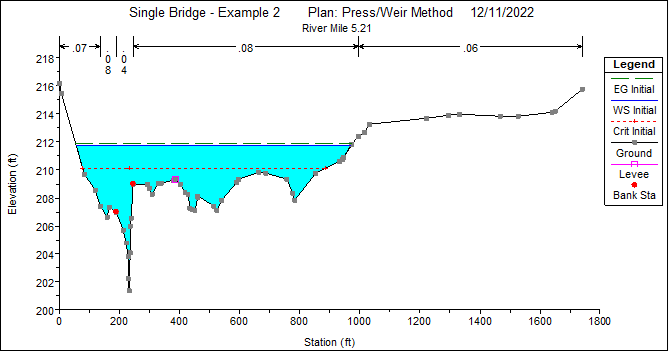
\includegraphics[scale=0.7, frame]{fig10.png}
    \\\emph{Figure 10: Cross Section for Initial $n$ Values of Station 5.21}\\
    \vspace{5mm}
    \addcontentsline{lof}{figure}{Figure 11: Cross Section for Halved $n$ Values of Station 5.21}
    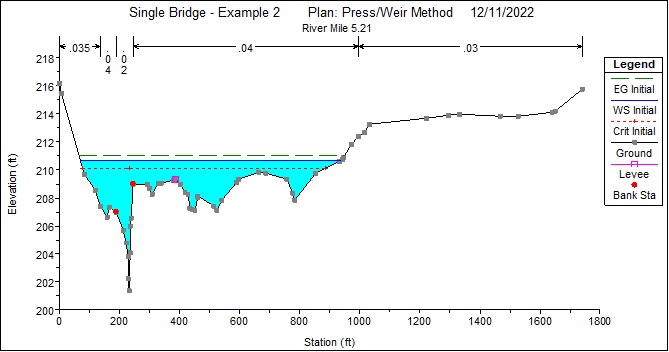
\includegraphics[scale=0.7, frame]{fig11.png}
    \\\emph{Figure 11: Cross Section for Halved $n$ Values of Station 5.21}\\
    \vspace{5mm}
    \addcontentsline{lof}{figure}{Figure 12: Cross Section for Doubled $n$ Values of Station 5.21}
    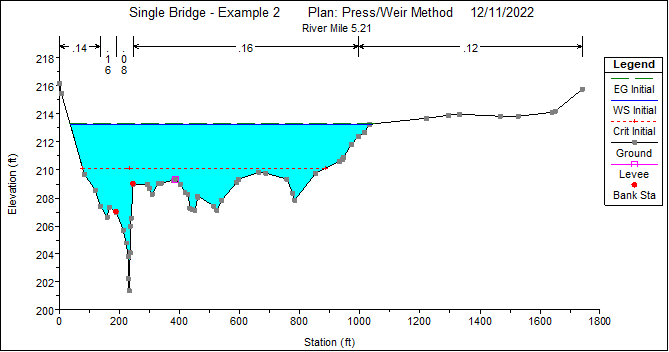
\includegraphics[scale=0.7, frame]{fig12.png}
    \\\emph{Figure 12: Cross Section for Doubled $n$ Values of Station 5.21}
\end{center}

% Station 5.065 Initial

\subsubsection{Station 5.065}
\begin{center}

\addcontentsline{lot}{table}{Table 16: Initial $n$ Values for Station 5.065}
\begin{tabular}{|cccc||cccc||cc|} 
    \hline
    \multicolumn{2}{|c}{\textbf{Fill }} & \multicolumn{2}{c||}{\textbf{Ground }} & \multicolumn{2}{c}{\textbf{Fill (cont'd) }} & \multicolumn{2}{c||}{\textbf{Ground (cont'd) }} & \multicolumn{2}{c|}{\textbf{Levee }}           \\ 
    \hline
    x        & y                        & x     & y                             & x     & y                                   & x      & y                                     & x        & y                                   \\
    109.3824 & 210.2814                 & 0     & 214.45                        & 417.3 & 208.31                              & 681.4  & 207.28                                & 365.5    & 208.6                               \\
    1119.114 & 210.2814                 & 11.1  & 213.86                        & 412.9 & 208.53                              & 695.9  & 207.66                                &          &                                     \\
    1107.9   & 210.14                   & 39    & 212.26                        & 365.5 & 208.6                               & 722.8  & 207.77                                & \multicolumn{2}{c|}{\textbf{Bank Station }}    \\ 
    \cline{9-10}
    1096.7   & 209.9                    & 41.1  & 211.82                        & 328.9 & 205.36                              & 724.1  & 207.78                                & x        & y                                   \\
    1078.9   & 209.59                   & 141.4 & 209.56                        & 328.9 & 203.41                              & 739.4  & 207.54                                & 274.5    & 205.05                              \\
    1076     & 209.5                    & 173.5 & 208.02                        & 316.3 & 202.12                              & 763.2  & 208.11                                & 365.5    & 208.6                               \\
    1055.3   & 209.77                   & 274.5 & 205.05                        & 312.8 & 200.76                              & 787    & 209.07                                &          &                                     \\
    998.3    & 209.75                   & 292.9 & 203.86                        & 307   & 199.9                               & 816    & 209.31                                & \multicolumn{2}{c|}{\textbf{Water Surface }}   \\ 
    \cline{9-10}
    970.4    & 209.81                   & 297.1 & 201.55                        & 299.3 & 201.33                              & 919.6  & 210.04                                & x        & y                                   \\
    919.6    & 210.04                   & 299.3 & 201.33                        & 297.1 & 201.55                              & 970.4  & 209.81                                & 109.3824 & 210.2814                            \\
    816      & 209.31                   & 307   & 199.9                         & 292.9 & 203.86                              & 998.3  & 209.75                                & 1119.114 & 210.2814                            \\
    787      & 209.07                   & 312.8 & 200.76                        & 274.5 & 205.05                              & 1055.3 & 209.77                                & 307      & 210.2814                            \\
    763.2    & 208.11                   & 316.3 & 202.12                        & 173.5 & 208.02                              & 1076   & 209.5                                 &          &                                     \\
    739.4    & 207.54                   & 328.9 & 203.41                        & 141.4 & 209.56                              & 1078.9 & 209.59                                & \multicolumn{2}{c|}{\textbf{Energy Grade }}    \\ 
    \cline{9-10}
    724.1    & 207.78                   & 328.9 & 205.36                        &       &                                     & 1096.7 & 209.9                                 & x        & y                                   \\
    722.8    & 207.77                   & 365.5 & 208.6                         &       &                                     & 1107.9 & 210.14                                & 97.48218 & 210.5496                            \\
    695.9    & 207.66                   & 412.9 & 208.53                        &       &                                     & 1130.1 & 210.42                                & 1218.028 & 210.5496                            \\
    681.4    & 207.28                   & 417.3 & 208.31                        &       &                                     & 1225.1 & 210.56                                & 307      & 210.5496                            \\
    667.1    & 206.76                   & 429.3 & 206.24                        &       &                                     & 1358.3 & 211.08                                &          &                                     \\
    650.7    & 205.84                   & 433.9 & 205.81                        &       &                                     & 1372.2 & 211.13                                & \multicolumn{2}{c|}{\textbf{Critical Level }}  \\ 
    \cline{9-10}
    644.1    & 205.93                   & 441.1 & 203.43                        &       &                                     & 1418.8 & 211.28                                & x        & y                                   \\
    638.1    & 205.98                   & 447.3 & 206.25                        &       &                                     & 1426.1 & 210.55                                & 161.41   & 208.6                               \\
    624.4    & 205.92                   & 448.6 & 206.36                        &       &                                     & 1442.6 & 211.38                                & 775.3483 & 208.6                               \\
    587.1    & 206.61                   & 487.7 & 208.09                        &       &                                     & 1472.3 & 211.49                                & 307      & 208.6                               \\
    584.9    & 206.68                   & 501.8 & 208.05                        &       &                                     & 1646.7 & 211.48                                &          &                                     \\
    575.3    & 205.82                   & 505.7 & 208.08                        &       &                                     & 1669.5 & 211.47                                &          &                                     \\
    566.4    & 205.95                   & 550.1 & 207.01                        &       &                                     & 1745.1 & 211.67                                &          &                                     \\
    565.6    & 205.95                   & 558.8 & 206.08                        &       &                                     & 1796.2 & 212.21                                &          &                                     \\
    558.8    & 206.08                   & 565.6 & 205.95                        &       &                                     & 1868.3 & 213.44                                &          &                                     \\
    550.1    & 207.01                   & 566.4 & 205.95                        &       &                                     & 1888   & 214.2                                 &          &                                     \\
    505.7    & 208.08                   & 575.3 & 205.82                        &       &                                     &        &                                       &          &                                     \\
    501.8    & 208.05                   & 584.9 & 206.68                        &       &                                     &        &                                       &          &                                     \\
    487.7    & 208.09                   & 587.1 & 206.61                        &       &                                     &        &                                       &          &                                     \\
    448.6    & 206.36                   & 624.4 & 205.92                        &       &                                     &        &                                       &          &                                     \\
    447.3    & 206.25                   & 638.1 & 205.98                        &       &                                     &        &                                       &          &                                     \\
    441.1    & 203.43                   & 644.1 & 205.93                        &       &                                     &        &                                       &          &                                     \\
    433.9    & 205.81                   & 650.7 & 205.84                        &       &                                     &        &                                       &          &                                     \\
    429.3    & 206.24                   & 667.1 & 206.76                        &       &                                     &        &                                       &          &                                     \\
    \hline\multicolumn{10}{c}{\emph{Table 16: Initial $n$ Values for Station 5.065}}
\end{tabular}

% Station 5.065 Halved

\addcontentsline{lot}{table}{Table 17: Halved $n$ Values for Station 5.065}
\begin{tabular}{|cccc||cc||cc|} 
    \hline
    \multicolumn{2}{|c}{\textbf{Fill }} & \multicolumn{2}{c||}{\textbf{Ground }} & \multicolumn{2}{c||}{\textbf{Ground (cont'd) }} & \multicolumn{2}{c|}{\textbf{Levee }}           \\ 
    \hline
    x        & y                        & x     & y                             & x      & y                                     & x        & y                                   \\
    137.5678 & 209.6463                 & 0     & 214.45                        & 998.3  & 209.75                                & 365.5    & 208.6                               \\
    863.7343 & 209.6463                 & 11.1  & 213.86                        & 1055.3 & 209.77                                &          &                                     \\
    816      & 209.31                   & 39    & 212.26                        & 1076   & 209.5                                 & \multicolumn{2}{c|}{\textbf{Bank Station }}    \\ 
    \cline{7-8}
    787      & 209.07                   & 41.1  & 211.82                        & 1078.9 & 209.59                                & x        & y                                   \\
    763.2    & 208.11                   & 141.4 & 209.56                        & 1096.7 & 209.9                                 & 274.5    & 205.05                              \\
    739.4    & 207.54                   & 173.5 & 208.02                        & 1107.9 & 210.14                                & 365.5    & 208.6                               \\
    724.1    & 207.78                   & 274.5 & 205.05                        & 1130.1 & 210.42                                &          &                                     \\
    722.8    & 207.77                   & 292.9 & 203.86                        & 1225.1 & 210.56                                & \multicolumn{2}{c|}{\textbf{Water Surface }}   \\ 
    \cline{7-8}
    695.9    & 207.66                   & 297.1 & 201.55                        & 1358.3 & 211.08                                & x        & y                                   \\
    681.4    & 207.28                   & 299.3 & 201.33                        & 1372.2 & 211.13                                & 137.5678 & 209.6463                            \\
    667.1    & 206.76                   & 307   & 199.9                         & 1418.8 & 211.28                                & 863.7343 & 209.6463                            \\
    650.7    & 205.84                   & 312.8 & 200.76                        & 1426.1 & 210.55                                & 1064.78  & 209.6463                            \\
    644.1    & 205.93                   & 316.3 & 202.12                        & 1442.6 & 211.38                                & 1082.136 & 209.6463                            \\
    638.1    & 205.98                   & 328.9 & 203.41                        & 1472.3 & 211.49                                & 307      & 209.6463                            \\
    624.4    & 205.92                   & 328.9 & 205.36                        & 1646.7 & 211.48                                &          &                                     \\
    587.1    & 206.61                   & 365.5 & 208.6                         & 1669.5 & 211.47                                & \multicolumn{2}{c|}{\textbf{Energy Grade }}    \\ 
    \cline{7-8}
    584.9    & 206.68                   & 412.9 & 208.53                        & 1745.1 & 211.67                                & x        & y                                   \\
    575.3    & 205.82                   & 417.3 & 208.31                        & 1796.2 & 212.21                                & 120.4322 & 210.0325                            \\
    566.4    & 205.95                   & 429.3 & 206.24                        & 1868.3 & 213.44                                & 918.5302 & 210.0325                            \\
    565.6    & 205.95                   & 433.9 & 205.81                        & 1888   & 214.2                                 & 921.2649 & 210.0325                            \\
    558.8    & 206.08                   & 441.1 & 203.43                        &        &                                       & 1102.881 & 210.0325                            \\
    550.1    & 207.01                   & 447.3 & 206.25                        &        &                                       & 307      & 210.0325                            \\
    505.7    & 208.08                   & 448.6 & 206.36                        &        &                                       &          &                                     \\
    501.8    & 208.05                   & 487.7 & 208.09                        &        &                                       & \multicolumn{2}{c|}{\textbf{Critical Level }}  \\ 
    \cline{7-8}
    487.7    & 208.09                   & 501.8 & 208.05                        &        &                                       & x        & y                                   \\
    448.6    & 206.36                   & 505.7 & 208.08                        &        &                                       & 161.41   & 208.6                               \\
    447.3    & 206.25                   & 550.1 & 207.01                        &        &                                       & 775.3483 & 208.6                               \\
    441.1    & 203.43                   & 558.8 & 206.08                        &        &                                       & 307      & 208.6                               \\
    433.9    & 205.81                   & 565.6 & 205.95                        &        &                                       &          &                                     \\
    429.3    & 206.24                   & 566.4 & 205.95                        &        &                                       &          &                                     \\
    417.3    & 208.31                   & 575.3 & 205.82                        &        &                                       &          &                                     \\
    412.9    & 208.53                   & 584.9 & 206.68                        &        &                                       &          &                                     \\
    365.5    & 208.6                    & 587.1 & 206.61                        &        &                                       &          &                                     \\
    328.9    & 205.36                   & 624.4 & 205.92                        &        &                                       &          &                                     \\
    328.9    & 203.41                   & 638.1 & 205.98                        &        &                                       &          &                                     \\
    316.3    & 202.12                   & 644.1 & 205.93                        &        &                                       &          &                                     \\
    312.8    & 200.76                   & 650.7 & 205.84                        &        &                                       &          &                                     \\
    307      & 199.9                    & 667.1 & 206.76                        &        &                                       &          &                                     \\
    299.3    & 201.33                   & 681.4 & 207.28                        &        &                                       &          &                                     \\
    297.1    & 201.55                   & 695.9 & 207.66                        &        &                                       &          &                                     \\
    292.9    & 203.86                   & 722.8 & 207.77                        &        &                                       &          &                                     \\
    274.5    & 205.05                   & 724.1 & 207.78                        &        &                                       &          &                                     \\
    173.5    & 208.02                   & 739.4 & 207.54                        &        &                                       &          &                                     \\
    141.4    & 209.56                   & 763.2 & 208.11                        &        &                                       &          &                                     \\
    1064.78  & 209.6463                 & 787   & 209.07                        &        &                                       &          &                                     \\
    1082.136 & 209.6463                 & 816   & 209.31                        &        &                                       &          &                                     \\
    1078.9   & 209.59                   & 919.6 & 210.04                        &        &                                       &          &                                     \\
    1076     & 209.5                    & 970.4 & 209.81                        &        &                                       &          &                                     \\
    \hline\multicolumn{8}{c}{\emph{Table 17: Halved $n$ Values for Station 5.065}}
\end{tabular}

%Station 5.065 Doubled

\addcontentsline{lot}{table}{Table 18: Doubled $n$ Values for Station 5.065}
\begin{tabular}{|cccc||cccc||cc|} 
    \hline
    \multicolumn{2}{|c}{\textbf{Fill}} & \multicolumn{2}{c||}{\textbf{Ground}} & \multicolumn{2}{c}{\textbf{Fill (cont'd)}} & \multicolumn{2}{c||}{\textbf{Ground (cont'd) }} & \multicolumn{2}{c|}{\textbf{Levee}}           \\ 
    \hline
    x        & y                       & x     & y                            & x     & y                                  & x      & y                                     & x        & y                                  \\
    58.87082 & 211.4196                & 0     & 214.45                       & 501.8 & 208.05                             & 681.4  & 207.28                                & 365.5    & 208.6                              \\
    1453.287 & 211.4196                & 11.1  & 213.86                       & 487.7 & 208.09                             & 695.9  & 207.66                                &          &                                    \\
    1442.6   & 211.38                  & 39    & 212.26                       & 448.6 & 206.36                             & 722.8  & 207.77                                & \multicolumn{2}{c|}{\textbf{Bank Station}}    \\ 
    \cline{9-10}
    1426.1   & 210.55                  & 41.1  & 211.82                       & 447.3 & 206.25                             & 724.1  & 207.78                                & x        & y                                  \\
    1418.8   & 211.28                  & 141.4 & 209.56                       & 441.1 & 203.43                             & 739.4  & 207.54                                & 274.5    & 205.05                             \\
    1372.2   & 211.13                  & 173.5 & 208.02                       & 433.9 & 205.81                             & 763.2  & 208.11                                & 365.5    & 208.6                              \\
    1358.3   & 211.08                  & 274.5 & 205.05                       & 429.3 & 206.24                             & 787    & 209.07                                &          &                                    \\
    1225.1   & 210.56                  & 292.9 & 203.86                       & 417.3 & 208.31                             & 816    & 209.31                                & \multicolumn{2}{c|}{\textbf{Water Surface}}   \\ 
    \cline{9-10}
    1130.1   & 210.42                  & 297.1 & 201.55                       & 412.9 & 208.53                             & 919.6  & 210.04                                & x        & y                                  \\
    1107.9   & 210.14                  & 299.3 & 201.33                       & 365.5 & 208.6                              & 970.4  & 209.81                                & 58.87082 & 211.4196                           \\
    1096.7   & 209.9                   & 307   & 199.9                        & 328.9 & 205.36                             & 998.3  & 209.75                                & 1453.287 & 211.4196                           \\
    1078.9   & 209.59                  & 312.8 & 200.76                       & 328.9 & 203.41                             & 1055.3 & 209.77                                & 307      & 211.4196                           \\
    1076     & 209.5                   & 316.3 & 202.12                       & 316.3 & 202.12                             & 1076   & 209.5                                 &          &                                    \\
    1055.3   & 209.77                  & 328.9 & 203.41                       & 312.8 & 200.76                             & 1078.9 & 209.59                                & \multicolumn{2}{c|}{\textbf{Energy Grade}}    \\ 
    \cline{9-10}
    998.3    & 209.75                  & 328.9 & 205.36                       & 307   & 199.9                              & 1096.7 & 209.9                                 & x        & y                                  \\
    970.4    & 209.81                  & 365.5 & 208.6                        & 299.3 & 201.33                             & 1107.9 & 210.14                                & 54.24223 & 211.5239                           \\
    919.6    & 210.04                  & 412.9 & 208.53                       & 297.1 & 201.55                             & 1130.1 & 210.42                                & 1689.866 & 211.5239                           \\
    816      & 209.31                  & 417.3 & 208.31                       & 292.9 & 203.86                             & 1225.1 & 210.56                                & 307      & 211.5239                           \\
    787      & 209.07                  & 429.3 & 206.24                       & 274.5 & 205.05                             & 1358.3 & 211.08                                &          &                                    \\
    763.2    & 208.11                  & 433.9 & 205.81                       & 173.5 & 208.02                             & 1372.2 & 211.13                                & \multicolumn{2}{c|}{\textbf{Critical Level}}  \\ 
    \cline{9-10}
    739.4    & 207.54                  & 441.1 & 203.43                       & 141.4 & 209.56                             & 1418.8 & 211.28                                & x        & y                                  \\
    724.1    & 207.78                  & 447.3 & 206.25                       &       &                                    & 1426.1 & 210.55                                & 161.41   & 208.6                              \\
    722.8    & 207.77                  & 448.6 & 206.36                       &       &                                    & 1442.6 & 211.38                                & 775.3483 & 208.6                              \\
    695.9    & 207.66                  & 487.7 & 208.09                       &       &                                    & 1472.3 & 211.49                                & 307      & 208.6                              \\
    681.4    & 207.28                  & 501.8 & 208.05                       &       &                                    & 1646.7 & 211.48                                &          &                                    \\
    667.1    & 206.76                  & 505.7 & 208.08                       &       &                                    & 1669.5 & 211.47                                &          &                                    \\
    650.7    & 205.84                  & 550.1 & 207.01                       &       &                                    & 1745.1 & 211.67                                &          &                                    \\
    644.1    & 205.93                  & 558.8 & 206.08                       &       &                                    & 1796.2 & 212.21                                &          &                                    \\
    638.1    & 205.98                  & 565.6 & 205.95                       &       &                                    & 1868.3 & 213.44                                &          &                                    \\
    624.4    & 205.92                  & 566.4 & 205.95                       &       &                                    & 1888   & 214.2                                 &          &                                    \\
    587.1    & 206.61                  & 575.3 & 205.82                       &       &                                    &        &                                       &          &                                    \\
    584.9    & 206.68                  & 584.9 & 206.68                       &       &                                    &        &                                       &          &                                    \\
    575.3    & 205.82                  & 587.1 & 206.61                       &       &                                    &        &                                       &          &                                    \\
    566.4    & 205.95                  & 624.4 & 205.92                       &       &                                    &        &                                       &          &                                    \\
    565.6    & 205.95                  & 638.1 & 205.98                       &       &                                    &        &                                       &          &                                    \\
    558.8    & 206.08                  & 644.1 & 205.93                       &       &                                    &        &                                       &          &                                    \\
    550.1    & 207.01                  & 650.7 & 205.84                       &       &                                    &        &                                       &          &                                    \\
    505.7    & 208.08                  & 667.1 & 206.76                       &       &                                    &        &                                       &          &                                    \\
    \hline\multicolumn{10}{c}{\emph{Table 18: Doubled $n$ Values for Station 5.065}}
\end{tabular}

\newpage\begin{center}
    \addcontentsline{lof}{figure}{Figure 13: Cross Section for Initial $n$ Values of Station 5.065}
    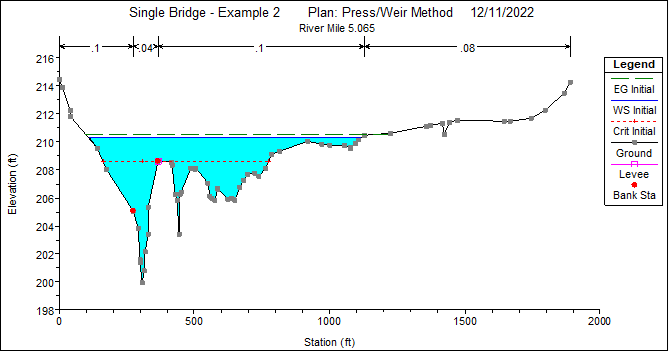
\includegraphics[scale=0.7, frame]{fig13.png}
    \\\emph{Figure 13: Cross Section for Initial $n$ Values of Station 5.065}\\
    \vspace{5mm}
    \addcontentsline{lof}{figure}{Figure 14: Cross Section for Halved $n$ Values of Station 5.065}
    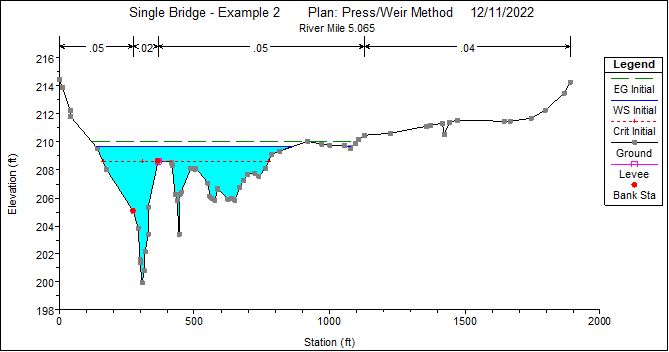
\includegraphics[scale=0.7, frame]{fig14.png}
    \\\emph{Figure 14: Cross Section for Halved $n$ Values of Station 5.065}\\
    \vspace{5mm}
    \addcontentsline{lof}{figure}{Figure 15: Cross Section for Doubled $n$ Values of Station 5.065}
    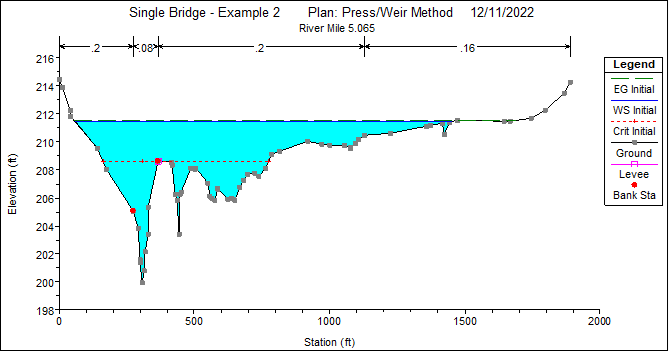
\includegraphics[scale=0.7, frame]{fig15.png}
    \\\emph{Figure 15: Cross Section for Doubled $n$ Values of Station 5.065}\\
\end{center}\newpage

\end{center}
\subsection{Varying Flows}
\subsubsection{Station 5.99}
\begin{center}
% 5.99 Flow

\addcontentsline{lot}{table}{Table 19: Flow Values for Station 5.99}
\begin{tabular}{|cc|cc|cc|} 
    \hline
    \multicolumn{2}{|c|}{\textbf{Levee }}                    & \multicolumn{2}{c|}{\textbf{Raised Water Surface }}  & \multicolumn{2}{c|}{\textbf{Lowered Outer Water Surface~ }}  \\ 
    \hline
    x      & y                                               & x       & y                                          & x       & y                                                  \\
    866    & 214.80                                          & 17.49   & 218.96                                     & 9.35    & 220.00                                             \\
           &                                                 & 1082.59 & 218.96                                     & 1872.07 & 220.00                                             \\
    \multicolumn{2}{|c|}{\textbf{Bank Station }}             & 1117.28 & 218.96                                     & 932.00  & 220.00                                             \\ 
    \cline{1-2}
    x      & y                                               & 1833.29 & 218.96                                     &         &                                                    \\
    866    & 214.80                                          & 932.00  & 218.96                                     & \multicolumn{2}{c|}{\textbf{Lowered Water Surface }}         \\ 
    \cline{5-6}
    948    & 216.60                                          &         &                                            & x       & y                                                  \\
           &                                                 & \multicolumn{2}{c|}{\textbf{Raised Energy Grade }}   & 867.69  & 214.70                                             \\ 
    \cline{3-4}
    \multicolumn{2}{|c|}{\textbf{Initial Water Surface }}    & x       & y                                          & 943.45  & 214.70                                             \\ 
    \cline{1-2}
    x      & y                                               & 15.18   & 219.26                                     & 932.00  & 214.70                                             \\
    29.99  & 217.37                                          & 1844.29 & 219.26                                     &         &                                                    \\
    980.23 & 217.37                                          & 932.00  & 219.26                                     & \multicolumn{2}{c|}{\textbf{Lowered Energy Grade }}          \\ 
    \cline{5-6}
    932.00 & 217.37                                          &         &                                            & x       & y                                                  \\
           &                                                 & \multicolumn{2}{c|}{\textbf{Raised Critical Level }} & 547.36  & 214.97                                             \\ 
    \cline{3-4}
    \multicolumn{2}{|c|}{\textbf{Initial Energy Grade }}     & x       & y                                          & 944.12  & 214.97                                             \\ 
    \cline{1-2}
    x      & y                                               & 523.72  & 215.88                                     & 932.00  & 214.97                                             \\
    28.43  & 217.57                                          & 946.28  & 215.88                                     &         &                                                    \\
    988.56 & 217.57                                          & 932.00  & 215.88                                     & \multicolumn{2}{c|}{\textbf{Lowered Critical Level }}        \\ 
    \cline{5-6}
    932.00 & 217.57                                          &         &                                            & x       & y                                                  \\
           &                                                 &         &                                            & 885.30  & 212.80                                             \\
    \multicolumn{2}{|c|}{\textbf{Initial Critical Level }}   &         &                                            & 938.93  & 212.80                                             \\ 
    \cline{1-2}
    x      & y                                               &         &                                            & 932.00  & 212.80                                             \\
    551.70 & 214.81                                          &         &                                            &         &                                                    \\
    943.72 & 214.81                                          &         &                                            &         &                                                    \\
    932.00 & 214.81                                          &         &                                            &         &                                                    \\
    \hline\multicolumn{6}{c}{\emph{Table 19: Flow Values for Station 5.99}}
\end{tabular}
\vspace{5mm}
\begin{center}
    \addcontentsline{lof}{figure}{Figure 16: Cross Section for Varying Flows of Station 5.99}
    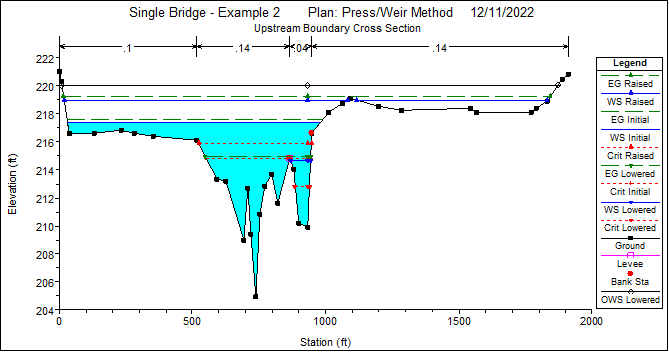
\includegraphics[scale=0.7, frame]{fig16.png}
    \\\emph{Figure 16: Cross Section for Varying Flows of Station 5.99}\\
\end{center}
\newpage

%5.76 Flow
\end{center}
    \subsubsection{Station 5.79}
\begin{center}
\addcontentsline{lot}{table}{Table 20: Flow Values for Station 5.76}
\begin{tabular}{|cc|cc|cc|} 
    \hline
    \multicolumn{2}{|c|}{\textbf{Levee }}                    & \multicolumn{2}{c|}{\textbf{Raised Water Surface }}  & \multicolumn{2}{c|}{\textbf{Lowered Outer Water Suface }}  \\ 
    \hline
    x        & y                                             & x        & y                                         & x        & y                                               \\
    906      & 214.3                                         & 31.14926 & 216.9803                                  & 8.000203 & 218.4                                           \\
             &                                               & 1663.011 & 216.9803                                  & 1767.353 & 218.4                                           \\
    \multicolumn{2}{|c|}{\textbf{Bank Station }}             & 423      & 216.9803                                  & 423      & 218.4                                           \\ 
    \cline{1-2}
    x        & y                                             &          &                                           &          &                                                 \\
    351      & 214.4                                         & \multicolumn{2}{c|}{\textbf{Raised Energy Grade }}   & \multicolumn{2}{c|}{\textbf{Lowered Energy Grade }}        \\ 
    \cline{3-6}
    548      & 212.7                                         & x        & y                                         & x        & y                                               \\
             &                                               & 29.17506 & 217.1262                                  & 369.5518 & 212.7351                                        \\
    \multicolumn{2}{|c|}{\textbf{Initial Water Surface }}    & 1672.301 & 217.1262                                  & 551.451  & 212.7351                                        \\ 
    \cline{1-2}
    x        & y                                             & 423      & 217.1262                                  & 423      & 212.7351                                        \\
    58.79404 & 215.1951                                      &          &                                           &          &                                                 \\
    1549.358 & 215.1951                                      & \multicolumn{2}{c|}{\textbf{Raised Critical Level }} & \multicolumn{2}{c|}{\textbf{Lowered Water Surface }}       \\ 
    \cline{3-6}
    423      & 215.1951                                      & x        & y                                         & x        & y                                               \\
             &                                               & 73.49975 & 214.3                                     & 370.5986 & 212.6411                                        \\
    \multicolumn{2}{|c|}{\textbf{~Initial Energy Grade }}    & 344.6444 & 214.3                                     & 547.4114 & 212.6411                                        \\ 
    \cline{1-2}
    x        & y                                             & 352.114  & 214.3                                     & 423      & 212.6411                                        \\
    56.87808 & 215.3118                                      & 1071.854 & 214.3                                     &          &                                                 \\
    1556.783 & 215.3118                                      & 1081.545 & 214.3                                     & \multicolumn{2}{c|}{\textbf{Lowered Critical Level }}      \\ 
    \cline{5-6}
    423      & 215.3118                                      & 1422.668 & 214.3                                     & x        & y                                               \\
             &                                               & 1449.199 & 214.3                                     & 395.2366 & 209.2168                                        \\
    \multicolumn{2}{|c|}{\textbf{Initial Critical Level }}   & 1492.368 & 214.3                                     & 437.4756 & 209.2168                                        \\ 
    \cline{1-2}
    x        & y                                             & 423      & 214.3                                     & 423      & 209.2168                                        \\
    145.7765 & 213.394                                       &          &                                           &          &                                                 \\
    287.0461 & 213.394                                       &          &                                           &          &                                                 \\
    362.2098 & 213.394                                       &          &                                           &          &                                                 \\
    616.242  & 213.394                                       &          &                                           &          &                                                 \\
    423      & 213.394                                       &          &                                           &          &                                                 \\
    \hline\multicolumn{6}{c}{\emph{Table 20: Flow Values for Station 5.76}}
    \end{tabular}
    \vspace{5mm}
    \begin{center}
        \addcontentsline{lof}{figure}{Figure 17: Cross Section for Varying Flows of Station 5.76}
        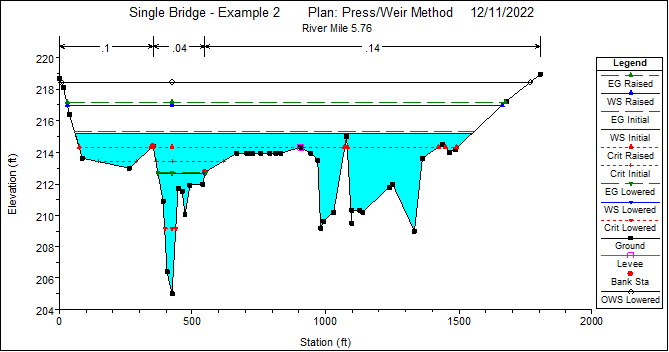
\includegraphics[scale=0.7, frame]{fig17.png}
        \\\emph{Figure 17: Cross Section for Varying Flows of Station 5.76}\\
    \end{center}

\newpage
\end{center}
    \subsubsection{Station 5.39}
\begin{center}
\addcontentsline{lot}{table}{Table 21: Flow Values for Station 5.39}
    \begin{tabular}{|cc|cc|cc|} 
        \hline
        \multicolumn{2}{|c|}{\textbf{Levee }}                    & \multicolumn{2}{c|}{\textbf{Raised Water Surface~ }} & \multicolumn{2}{c|}{\textbf{Lowered Outer Water Surface~ }}  \\ 
        \hline
        x        & y                                             & x        & y                                         & x        & y                                                 \\
        420      & 211.1329                                      & 66.58905 & 214.4058                                  & 44.50021 & 215.2                                             \\
        420      & 215                                           & 1629.991 & 214.4058                                  & 1705     & 215.2                                             \\
        677      & 212.4333                                      & 548.4    & 214.4058                                  & 548.4    & 215.2                                             \\
        677      & 215                                           &          &                                           &          &                                                   \\
                 &                                               & \multicolumn{2}{c|}{\textbf{Raised Energy Grade }}   & \multicolumn{2}{c|}{\textbf{Lowered Water Surface~ }}        \\ 
        \cline{3-6}
        \multicolumn{2}{|c|}{\textbf{Bank Station }}             & x        & y                                         & x        & y                                                 \\ 
        \cline{1-2}
        x        & y                                             & 46.65439 & 215.1225                                  & 175.4502 & 211.8853                                          \\
        450      & 213.4                                         & 1698.029 & 215.1225                                  & 365.9035 & 211.8853                                          \\
        647      & 213.5                                         & 548.4    & 215.1225                                  & 368.0163 & 211.8853                                          \\
                 &                                               &          &                                           & 445.9219 & 211.8853                                          \\
        \multicolumn{2}{|c|}{\textbf{Initial Water Surface~ }}   & \multicolumn{2}{c|}{\textbf{Raised Critical Level~ }}      & 459.0977 & 211.8853                                          \\ 
        \cline{1-4}
        x        & y                                             & x        & y                                         & 637.9921 & 211.8853                                          \\
        132.172  & 212.7437                                      & 257.4308 & 210.947                                   & 1060.266 & 211.8853                                          \\
        448.233  & 212.7437                                      & 295.9608 & 210.947                                   & 1428.527 & 211.8853                                          \\
        456.9847 & 212.7437                                      & 432.8412 & 210.947                                   & 548.4    & 211.8853                                          \\
        642.2935 & 212.7437                                      & 443.3959 & 210.947                                   &          &                                                   \\
        668.2709 & 212.7437                                      & 462.6731 & 210.947                                   & \multicolumn{2}{c|}{\textbf{Lowered Energy Grade }}          \\ 
        \cline{5-6}
        815.742  & 212.7437                                      & 633.0356 & 210.947                                   & x        & y                                                 \\
        991.0397 & 212.7437                                      & 1103.187 & 210.947                                   & 174.6255 & 211.9016                                          \\
        1463.4   & 212.7437                                      & 1225.339 & 210.947                                   & 445.966  & 211.9016                                          \\
        548.4    & 212.7437                                      & 1254.218 & 210.947                                   & 459.0575 & 211.9016                                          \\
                 &                                               & 1344.628 & 210.947                                   & 638.1121 & 211.9016                                          \\
        \multicolumn{2}{|c|}{\textbf{Initial Energy Grade }}     & 548.4    & 210.947                                   & 691.9537 & 211.9016                                          \\ 
        \cline{1-2}
        x        & y                                             &          &                                           & 692.2417 & 211.9016                                          \\
        116.9662 & 213.0453                                      &          &                                           & 1057.376 & 211.9016                                          \\
        449.0451 & 213.0453                                      &          &                                           & 1429.192 & 211.9016                                          \\
        454.6819 & 213.0453                                      &          &                                           & 548.4    & 211.9016                                          \\
        643.3994 & 213.0453                                      &          &                                           &          &                                                   \\
        659.7883 & 213.0453                                      &          &                                           & \multicolumn{2}{c|}{\textbf{Lowered Critical Level~ }}      \\ 
        \cline{5-6}
        859.3232 & 213.0453                                      &          &                                           & x        & y                                                 \\
        971.184  & 213.0453                                      &          &                                           & 517.6659 & 205.2723                                          \\
        1475.653 & 213.0453                                      &          &                                           & 592.817  & 205.2723                                          \\
        548.4    & 213.0453                                      &          &                                           & 548.4    & 205.2723                                          \\
                 &                                               &          &                                           &          &                                                   \\
        \multicolumn{2}{|c|}{\textbf{Initial Critical Level}}    &          &                                           &          &                                                   \\ 
        \cline{1-2}
        x        & y                                             &          &                                           &          &                                                   \\
        476.0116 & 208.9116                                      &          &                                           &          &                                                   \\
        618.6844 & 208.9116                                      &          &                                           &          &                                                   \\
        548.4    & 208.9116                                      &          &                                           &          &                                                   \\
        \hline\multicolumn{6}{c}{\emph{Table 21: Flow Values for Station 5.39}}
        \end{tabular}

        \begin{center}
            \addcontentsline{lof}{figure}{Figure 18: Cross Section for Varying Flows of Station 5.39}
            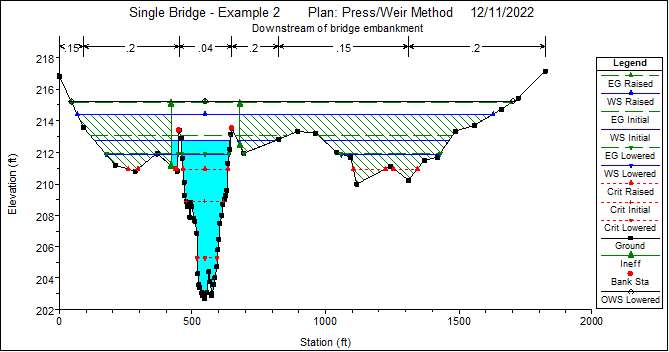
\includegraphics[scale=0.7, frame]{fig18.png}
            \\\emph{Figure 18: Cross Section for Varying Flows of Station 5.39}\\
        \end{center}
        \newpage
    \end{center}
            \subsubsection{Station 5.21}
        \begin{center}
        \addcontentsline{lot}{table}{Table 22: Flow Values for Station 5.21}
        \begin{tabular}{|cc|cc|cc|} 
            \hline
            \multicolumn{2}{|c|}{\textbf{Levee }}                    & \multicolumn{2}{c|}{\textbf{Raised Water Surface~ }}  & \multicolumn{2}{c|}{\textbf{Lowered Water Surface~ }}  \\ 
            \hline
            x        & y                                             & x        & y                                          & x        & y                                           \\
            383.6    & 209.29                                        & 32.45682 & 213.4492                                   & 54.37818 & 211.8307                                    \\
                     &                                               & 1122.559 & 213.4492                                   & 974.7261 & 211.8307                                    \\
            \multicolumn{2}{|c|}{\textbf{Bank Station }}             & 231.5    & 213.4492                                   & 231.5    & 211.8307                                    \\ 
            \cline{1-2}
            x        & y                                             &          &                                            &          &                                             \\
            189      & 206.95                                        & \multicolumn{2}{c|}{\textbf{Raised Energy Grade }}    & \multicolumn{2}{c|}{\textbf{Lowered Energy Grade }}    \\ 
            \cline{3-6}
            246      & 208.95                                        & x        & y                                          & x        & y                                           \\
                     &                                               & 30.35671 & 213.6043                                   & 54.31536 & 211.8353                                    \\
            \multicolumn{2}{|c|}{\textbf{Initial Water Surface~ }}   & 1185.627 & 213.6043                                   & 974.9108 & 211.8353                                    \\ 
            \cline{1-2}
            x        & y                                             & 231.5    & 213.6043                                   & 231.5    & 211.8353                                    \\
            55.56815 & 211.7428                                      &          &                                            &          &                                             \\
            972.1729 & 211.7428                                      & \multicolumn{2}{c|}{\textbf{Raised Critical Level~ }} & \multicolumn{2}{c|}{\textbf{Lowered Critical Level }}  \\ 
            \cline{3-6}
            231.5    & 211.7428                                      & x        & y                                          & x        & y                                           \\
                     &                                               & 64.83223 & 211.0588                                   & 133.3764 & 207.6068                                    \\
            \multicolumn{2}{|c|}{\textbf{Initial Energy Grade }}     & 952.3505 & 211.0588                                   & 241.5979 & 207.6068                                    \\ 
            \cline{1-2}
            x        & y                                             & 231.5    & 211.0588                                   & 231.5    & 207.6068                                    \\
            53.87888 & 211.8675                                      &          &                                            &          &                                             \\
            976.194  & 211.8675                                      &          &                                            &          &                                             \\
            231.5    & 211.8675                                      &          &                                            &          &                                             \\
                     &                                               &          &                                            &          &                                             \\
            \multicolumn{2}{|c|}{\textbf{Initial Critical Level}}    &          &                                            &          &                                             \\ 
            \cline{1-2}
            x        & y                                             &          &                                            &          &                                             \\
            77.36282 & 210.1336                                      &          &                                            &          &                                             \\
            887.7552 & 210.1336                                      &          &                                            &          &                                             \\
            231.5    & 210.1336                                      &          &                                            &          &                                             \\
            \hline\multicolumn{6}{c}{\emph{Table 22: Flow Values for Station 5.21}}
            \end{tabular}
            \vspace{5mm}
            \begin{center}
                \addcontentsline{lof}{figure}{Figure 19: Cross Section for Varying Flows of Station 5.21}
                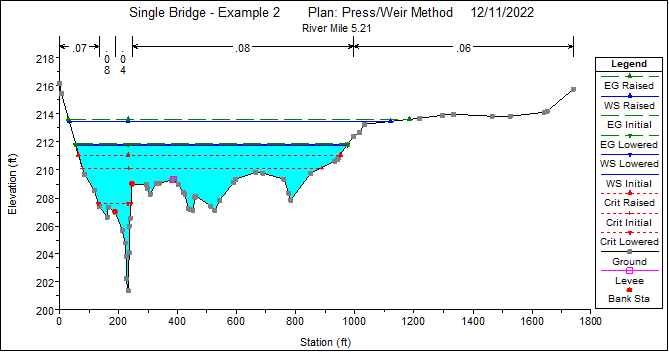
\includegraphics[scale=0.7, frame]{fig19.png}
                \\\emph{Figure 19: Cross Section for Varying Flows of Station 5.21}\\
            \end{center}
            \newpage
        \end{center}
                \subsubsection{Station 5.065}
            \begin{center}
            \addcontentsline{lot}{table}{Table 23: Flow Values for Station 5.065}
            \begin{tabular}{|cc|cc|cc|} 
                \hline
                \multicolumn{2}{|c|}{\textbf{Levee}}                    & \multicolumn{2}{c|}{\textbf{Raised Water Surface~}} & \multicolumn{2}{c|}{\textbf{Lowered Outer Water Surface~}}  \\ 
                \hline
                x        & y                                            & x        & y                                        & x        & y                                                \\
                365.5    & 208.6                                        & 48.87888 & 211.6447                                 & 34.81492 & 212.5                                            \\
                         &                                              & 1735.548 & 211.6447                                 & 1813.199 & 212.5                                            \\
                \multicolumn{2}{|c|}{\textbf{Bank Station}}             & 307      & 211.6447                                 & 307      & 212.5                                            \\ 
                \cline{1-2}
                x        & y                                            &          &                                          &          &                                                  \\
                274.5    & 205.05                                       & \multicolumn{2}{c|}{\textbf{Raised Energy Grade}}   & \multicolumn{2}{c|}{\textbf{Lowered Water Surface~}}        \\ 
                \cline{3-6}
                365.5    & 208.6                                        & x        & y                                        & x        & y                                                \\
                         &                                              & 40.2533  & 211.9974                                 & 41.80428 & 211.8041                                         \\
                \multicolumn{2}{|c|}{\textbf{Initial Water Surface~}}   & 1776.082 & 211.9974                                 & 1757.793 & 211.8041                                         \\ 
                \cline{1-2}
                x        & y                                            & 307      & 211.9974                                 & 307      & 211.8041                                         \\
                109.3824 & 210.2814                                     &          &                                          &          &                                                  \\
                1119.114 & 210.2814                                     & \multicolumn{2}{c|}{\textbf{Raised Critical Level}} & \multicolumn{2}{c|}{\textbf{Lowered Energy Grade}}          \\ 
                \cline{3-6}
                307      & 210.2814                                     & x        & y                                        & x        & y                                                \\
                         &                                              & 135.4191 & 209.6948                                 & 41.66681 & 211.8072                                         \\
                \multicolumn{2}{|c|}{\textbf{Initial Energy Grade}}     & 870.6054 & 209.6948                                 & 1758.087 & 211.8072                                         \\ 
                \cline{1-2}
                x        & y                                            & 1061.068 & 209.6948                                 & 307      & 211.8072                                         \\
                97.48218 & 210.5496                                     & 1084.916 & 209.6948                                 &          &                                                  \\
                1218.028 & 210.5496                                     & 307      & 209.6948                                 & \multicolumn{2}{c|}{\textbf{Lowered Critical Level }}       \\ 
                \cline{5-6}
                307      & 210.5496                                     &          &                                          & x        & y                                                \\
                         &                                              &          &                                          & 279.3643 & 204.7354                                         \\
                \multicolumn{2}{|c|}{\textbf{Initial Critical Level}}   &          &                                          & 328.9    & 204.7354                                         \\ 
                \cline{1-2}
                x        & y                                            &          &                                          & 307      & 204.7354                                         \\
                161.41   & 208.6                                        &          &                                          &          &                                                  \\
                775.3483 & 208.6                                        &          &                                          &          &                                                  \\
                307      & 208.6                                        &          &                                          &          &                                                  \\
                \hline\multicolumn{6}{c}{\emph{Table 23: Flow Values for Station 5.065}}
                \end{tabular}
                \vspace{5mm}
                \begin{center}
                    \addcontentsline{lof}{figure}{Figure 20: Cross Section for Varying Flows of Station 5.065}
                    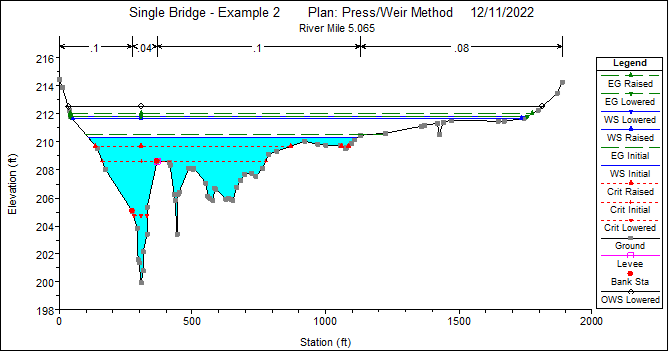
\includegraphics[scale=0.7, frame]{fig20.png}
                    \\\emph{Figure 20: Cross Section for Varying Flows of Station 5.065}\\
                \end{center}
\end{center}
    \newpage
    \section{Sample Calculations}
    \subsection{Percentages in Reductions}
    \[\%_{\text{Freeze}}=\frac{V_\text{Solid}}{V_\text{Total}}\times 100\]
    \[\text{Sample Calculation: }\%_{\text{Freeze}}=\frac{10\text{ mL}}{100\text{ mL}}\times 100=10\%\]
    \[\%_{\text{Centrifuge}}=\frac{V_\text{Centrate}}{V_\text{Centrate}+V_\text{Sludge}}\times 100\]
    \[\text{Sample Calculation: }=\frac{25\text{ mL}}{25\text{ mL}+75\text{ mL}}\times 100=25\%\]
    \subsection{Normalization}
    \[N=\frac{V_\text{Acid}}{V_\text{Total}}\times100\]
    \[\text{Sample Calculation: }N=\frac{0.1\text{ mL/L}\times100\text{ mL}}{155\text{ mL}}\times100=14.9\%\]
    \subsection{Relative Proportions}
    \[\%_{\text{SN}}=\frac{\text{Concentration}_\text{SN}}{\text{Concentration}_\text{SN}+\text{Concentration}_\text{SL}}\times 100\]
    \[\text{Sample Calculation: }\%_{\text{SN}}=\frac{\text{10\text{ mg/L}}}{\text{10\text{ mg/L}}+\text{40\text{ mg/L}}}\times 100=20\%\]
    \[\%_{\text{SL}}=\frac{\text{Concentration}_\text{SL}}{\text{Concentration}_\text{SN}+\text{Concentration}_\text{SL}}\times 100\]
    \[\text{Sample Calculation: }\%_{\text{SL}}=\frac{\text{40\text{ mg/L}}}{\text{10\text{ mg/L}}+\text{40\text{ mg/L}}}\times 100=80\%\]
    \newpage
    \section{Discussion}
    \subsection{Theory}
    \indent This experiment determines the percentage of lead removed from a municipal wastewater sample. This metric is crucial to public health since lead is one of seven toxic metals that are encountered in municipal wastewater. The encounter of these metals is disconcerting, but important, especially since they have effects that can devastate various species. After this metal is found, it can be treated in a wastewater facility. It's very important to treat wastewater as these metals will remain in the wastewater otherwise. Processes used to treat wastewater include reduction, conditioning, and dewatering.\\
    \indent Up to this point in the course, the importance of chemical and biological processes were emphasized. Both types of processes were crucial to this experiment. Acidification involves the chemical process of titration. The water is separated from the chemicals and the solids are digested. Freeze/thaw, acidification, and centrifugation are all chemical processes crucial to determining the percentage of lead removed from municipal sludge.\\
    \indent Overall, the three processes analyzed in this experiment are crucial to wastewater treatment facilities today. Today, America has more than 16,000 publicly-owned wastewater treatment facilities. All methods used in this experiment are used in every single one of those facilities, showing why these processes are crucial to the lives of every American.
    \subsection{Experimental}
    \indent As shown in \textit{Figure 1}, the municipal sludge went through three different processes. The first of the three was freeze/thaw. Originally, the sludge contained 98\% water and 2\% solids. After the freeze/thaw process, 65\% of the supernatant was poured off, which contained 99.6\% water and 0.4\% solids. The sludge sample that remained contained 94.9\% water and 5.1\% solids. The next process was acidification. After the acidification process, 55\% of the supernatant was poured off, which contained 96.4\% water and 3.6\% solids. The sludge sample that remained contained 91.7\% water and 8.3\% solids. The next and final process was centrifugation. After the centrifugation process, 75\% of the supernatant was poured off, which contained 76\% water and 24\% solids. The final remaining sludge was 3.9\% of the original sample, which can be disposed of safely following neutralization.\\
    \indent The next component of the experiment is acidification. Three acids were used to acidify the sludge sample: sulfuric acid, nitric acid, and acetic acid. The primary objective is to determine what acids are successful in reducing the pH of the sludge sample to 1.5. It's very important to lower the pH of municipal sludge as it makes the metals easier to be removed. The sulfuric acid was able to reduce the pH from 7.7 to 1.6 and the nitric acid was able to reduce the pH from 7.1 to 1.45. However, the acetic acid was unsuccessful in lowering the pH. The normalization became too high and the lowest the pH was throughout the titration was 3.6. It has been determined that acetic acid is not a candidate for the acidification process.\\
    \indent The final component of the experiment is centrifugation. There were four groups analyzed. Group A had the highest percentage removal of lead of 83.8\% at a mixing time of 20 hours with sulfuric acid with a pH of 1.5. Group D had the highest percentage removal of lead of 42.3\% at a mixing time of 6 hours with sulfuric acid with a pH of 1.5. From these results it is seen that a pH of 1.5 is most effective in the removal of lead.
    \newpage
    \section{Conclusions}
    \indent Following the treatment of the sludge, the sludge must be neutralized, since it has a pH of 1.5 and can harm the environment. The supernatant must also follow a similar treatment process. Neutralization allows for hte pH of any solution to be brought up to the pH of water (approximately 7) by titrating it with a basic chemical.\\
    \indent It has been determined from the experiment that the three processes of freeze/thaw, acidification, and centrifugation are all effective methods of treating municipal sludge. The freeze/thaw process allowed for 65\% of the supernatant to be poured off, the acidification process allowed for 55\% of the supernatant to be poured off, and the centrifugation process allowed for 75\% of the supernatant to be poured off. 3.9\% of the original sample remained and was made of 76\% water and 24\% solids.\\
    \indent It was shown in the acidification data that sulfuric acid and nitric acid are effective in reducing the pH of sludge to 1.5. acetic acid is not effective in doing so.\\ 
    \indent It was shown in the centrifugation data that the most effective method of removing lead was in Group A, with a mixing time of 20 hours and sulfuric acid with a pH of 1.5. It is also shown in Group D that 1.5 is an effective pH in removing lead. Using the three processes of freeze/thaw, acidification with either sulfuric or nitric acid, and centrifugation with a 1.5 pH sample of sulfuric acid are effective in removing metals from municipal sludge.
    \newpage
    \section{Questions}
    \begin{enumerate}
        \item Differentiate between and list systems of sludge management and ultimate sludge disposal.
        \\\rule{5cm}{1pt}
        \\\\Sludge management involves removing potentially reusable and recyclable materials from processed sludge. The systems include dewatering, digestion, and thickening. Ultimate sludge disposal involves discharging sludge that has already been treated. The systems include incineration, landfilling, and recycling.
        \item List all heavy metals that may be encountered in anaerobically digested municipal sludge and explain briefly why they are of concern and need to be removed to a larger or lesser extent.
        \\\rule{5cm}{1pt}
        \\\\The metals that may be encountered in anaerobically digested municipal sludge are Cadmium, Chromium, Copper, Mercury, Nickel, lead, and Zinc. These metals must be removed as they are harmful to humans if ingested. There are many affects, such as nausea, vomiting, and stomach pain. It also increases the risk of cancer.
        \item Assume that you have a 1\% by weight solution of a chemical. How do you prepare a 100 mg/L solution of this using distilled water and a 100-mL graduated cylinder? If you add 1 mL of this latter solution to a beaker with 200 mL of sample, what would the concentration of the chemical be, assuming there is not a trace of this chemical in the sample?
        \\\rule{5cm}{1pt}
        \[1\%=10000\text{ mg/L}=10\text{ mg/mL}\]
        \[\boxed{\text{To prepare a 100 mg/L solution, add 1 mL of solution to a 100 mL beaker of distilled water.}}\]
        \[\frac{1 \text{ mL}}{200 \text{ mL}}\times\frac{100 \text{ mL}}{1 \text{ L}}=\boxed{0.5 \text{ mg/L}}\]
        \item Say that you mix 100 mL of a 0.02\% solution of a chemical with 50 mL of a 500 mg/L solution of the same chemical. How many mL of the final solution do you need to add in 1 L of distilled water in order to produce a concentration of 1.5 mg/L?
        \\\rule{5cm}{1pt}
        \[0.02\%\times100\text{ mL}\times 10\text{ mg/mL}+50\text{ mL}\times 500\text{ mg/L}\times\frac{1\text{ L}}{1000\text{ mL}}=45\text{ mg}\]
        \[\frac{45\text{ mg}}{150\text{ mL}}=0.3\text{ mg/mL}=300\text{ mg/L}\]
        \[\frac{1.5\text{ mg/L}}{300\text{ mg/L}}\times1000\text{ mL}=\boxed{5\text{ mL}}\]
        \item You need to prepare a series of chlorine concentrations in 200-mL beakers of water samples to study the chlorine demand. What you have available is a bottle of commercial CLOROX (5.25\% by weight chlorine content) and several 100-mL graduated cylinders. To reduce the error, you want to make consecutive 100X or less dilutions, so that the last prepared solution will contain 1 mg/mL of chlorine. Describe the procedure and show your calculations.
        \\\rule{5cm}{1pt}
        \[0.0525\times x\text{ g CLOROX}\div 100\text{ mL H}_2\text{O}=1\text{ mg/mL}\]
        \[x=1904\text{ mg CLOROX}\]
        1904 mg CLOROX is needed to obtain a 1 mg/mL solution of chlorine. Add 1.9 mg of CLOROX to a 100 mL beaker of distilled water.
    \end{enumerate}
    \newpage
    \section{References}
    \begin{enumerate}
        \item McCarthy, P., and Sawyer, C. N., 1981, \underline{Chemistry for Environmental Engineers and Scientists}, 4th Ed., pp. 244-45, McGraw-Hill Book Company, New York, N.Y.
        \item Jones, J., Brown, K., and Hirsch, R., 1985, ``The Role of Phosphorus in Lake Eutrophication in New South Wales'', Water Research \underline{22} (2) 142.
        \item Prof. C. Yapijakis, Lecture Notes, CE-344: The Cooper Union School of Engineering.
        \item Adler, R.J., Jones, K.F., and Pappas, E.H. (1987). ``Sludge Disposal by Use of Pyrolysis'', J. Wat. Poll. Control Fed., \underline{58}, 6, pp. 3-12.
    \end{enumerate}
    
    \newpage
    
    
\end{document}